% !TeX root = MDA_VL_Ostermann_Folien.tex
% !TeX spellcheck = de_DE_frami

\begin{frame}
	\centering
	{\color{TUDoGreen} \huge\textbf{Hallo!}}\\
	\medskip
	\Large Ich bin \textbf{Fabian Ostermann}
	
	\bigskip
	\begin{itemize}
		\normalsize
		\item Doktorand bei Prof. Rudolph am LS\,11 (Computational Intelligence)\\
		\item B.Sc. und M.Sc. Informatik an der TU Dortmund\\
		\item Studium Jazzgitarre an der Folkwang Univ. Essen
		\item Forschung zu
		\begin{itemize}
			\item Computer Music
			\item Generative Artificial Intelligence
			\item Procedural Content Generation in Games
		\end{itemize}
	\end{itemize}
\end{frame}

%%%%%%%%%%%%%%%%%%%%%%%%%%%%%%%%%%%
%%%%%%%%%%%%%%%%%%%%%%%%%%%%%%%%%%%
\section{Einleitung und Motivation}

\begin{frame}[t]{Komposition}
{\enquote{Was ist das?}}
	%vgl. 24.2.1 What Composers Do
	%-> Rückgriff auf Ebelings Folien: Was ist Musik?
	
	\underline{Hiller und Issacson} (1959) formulieren pragmatisch:
	\begin{quote}
		\enquote{the act of composing can be thought of as the \textbf{extraction of order} out of a chaotic multitude of \textbf{available possibilities}} \citep[S.1]{HillerIssacson1959}
	\end{quote}
	
	\conclude~Also: \textbf{Suchproblem}
	\bigskip
	
	\questSign~Was könnte (sinnvoller) \emph{Suchraum} sein?
	
	\vspace{-.6cm}
	\hspace{-.3cm}
	\mbox{
		\raisebox{.5cm}{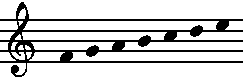
\includegraphics[height=1.2cm]{lily/Intro_pitches.pdf}}
		\raisebox{.5cm}{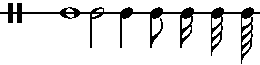
\includegraphics[height=.9cm]{lily/Intro_rhythms.pdf}}
		\raisebox{.2cm}{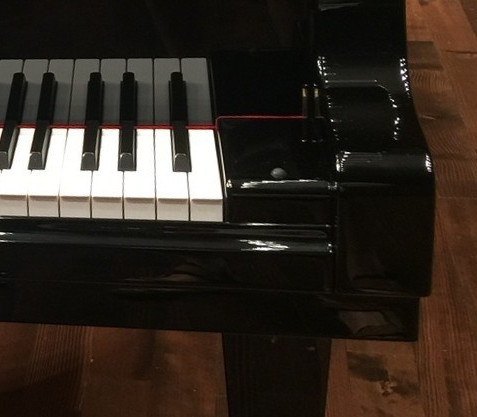
\includegraphics[height=2.1cm]{img/piano_edge.jpg}}
		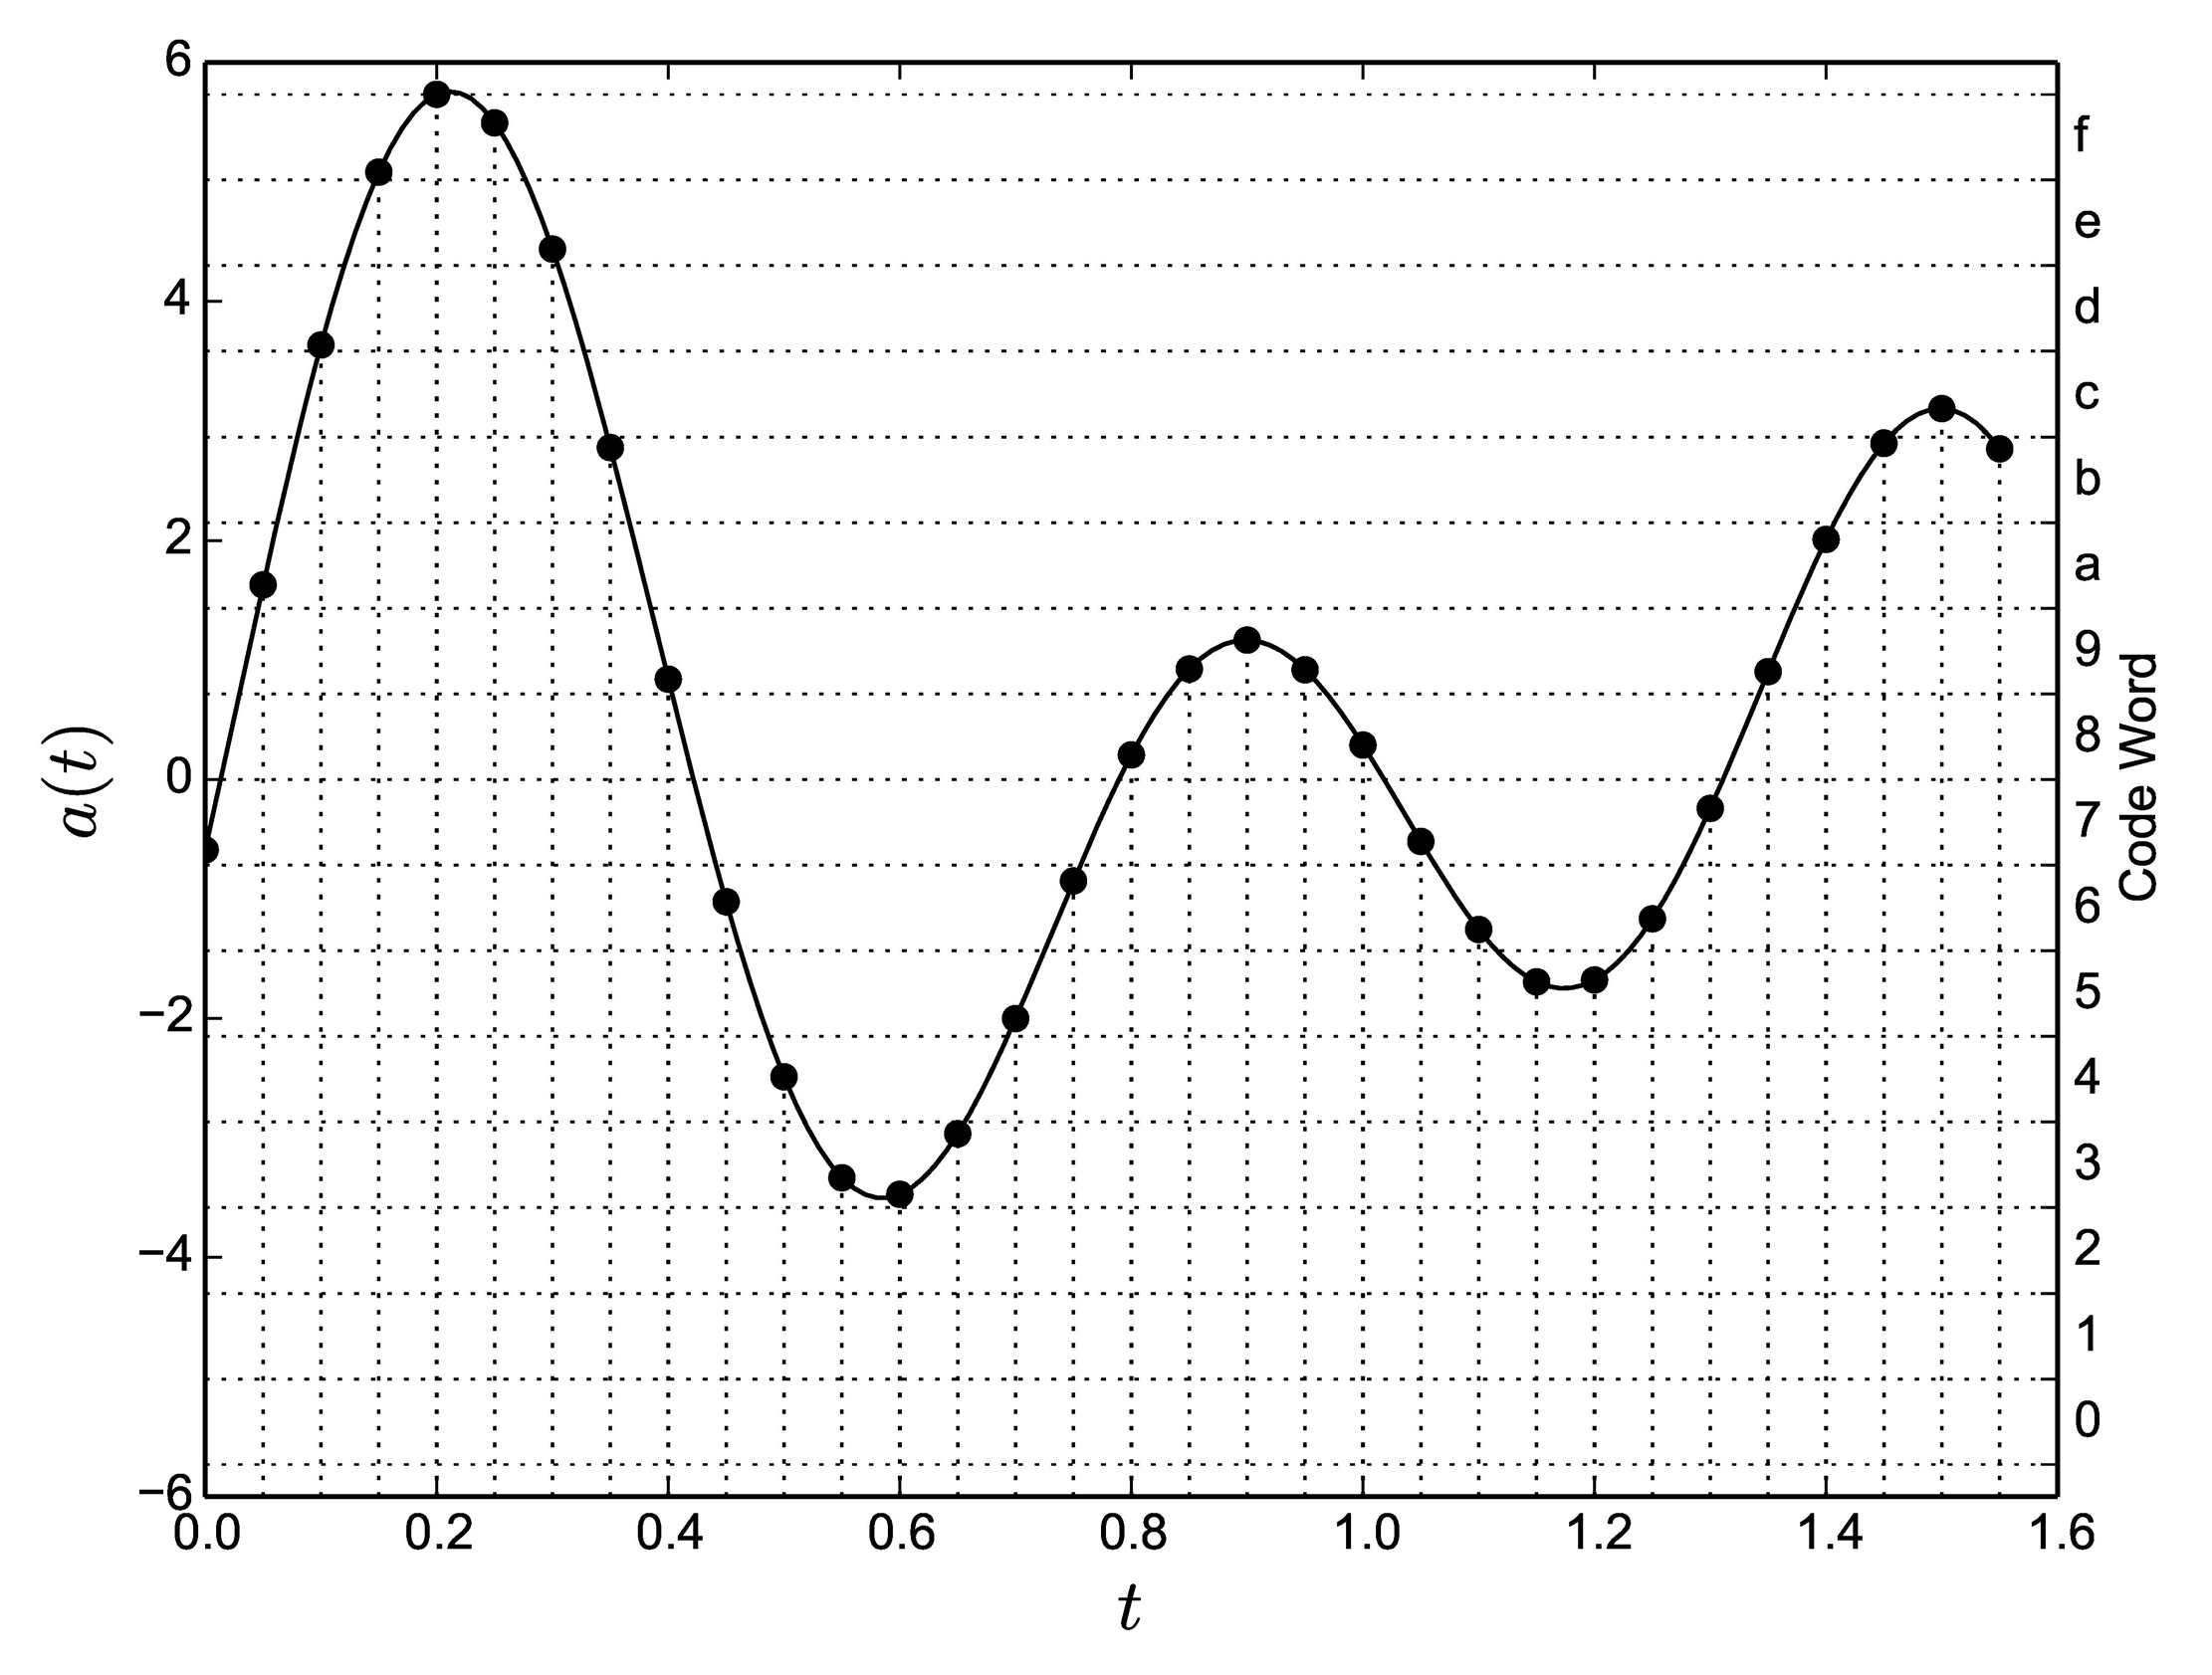
\includegraphics[height=2.6cm]{img/PCM_Waveform.png}
	}

	\medskip
	~~~~~~\conclude~Tonhöhe (Ton-Qualität), Lautstärke (Ton-Intensität), Dauer, Klangfarbe, ...\\\medskip
	~~~~~~~~~~~\Conclude~In jeden Fall sehr groß! (\emph{Combinatorial explosion})
\end{frame}

\begin{frame}[t]{Automatische Komposition}
{\enquote{Was ist das genau?}}
	
	\begin{multicols}{2}
		\newcommand{\pointerleft}{{\color{TUDoGreen}\Large$\blacktriangleleft$}}
	\begin{infobox}[.45\textwidth]{Begriffe}
		
		\textbf{Automat}isches Komponieren~~\visible<2>{\pointerleft}\\\medskip
		~~~vs.\\\medskip
		\textbf{Algorithm}isches Komponieren~~\visible<3>{\pointerleft}\\\medskip
		~~~vs.\\\medskip
		Computermusik~~\visible<4>{\pointerleft}
	\end{infobox}
	
	\columnbreak
	\only<2>{
		\begin{itemize}
			\item Autonome Maschine
			\item Vollautomatisch
			\item[\Conclude] Keine Eingabe oder Steuerung nötig
		\end{itemize}
	}
	\only<3>{
		\begin{itemize}
			\item[Def.] \emph{Algorithmus} = \enquote{eindeutige Handlungsvorschrift zur Lösung eines Problems}
			\item[\Conclude] \enquote{Generierung von musikalischem Material unter Einbeziehung \textbf{eindeutiger} Handlungsvorschriften}\\ \hfill{\citep[S.513]{FernandezVico2013}}
			\item Demnach: Von Menschen manuell durchführbar
		\end{itemize}
	}
	\only<4>{
		\begin{itemize}
			\item[\Conclude] \enquote{Jegliche Musik, in deren Entstehung ein Computer involviert war}
			\item Also heute \textbf{fast alles}!
			\item[Bsp.1:] Elektronische Musik per se
			\item[Bsp.2:] Traditionelle Musikproduktion mischen auf Digitalpulten
			\item[Bsp.3:] Klassische Komponisten schreiben Partituren in Notensatzprogrammen 
			\item[\Conclude] Begriff eher \textbf{unbrauchbar}
		\end{itemize}
	}
	\end{multicols}

\end{frame}

\begin{frame}[t]{Motivation}
{\enquote{Warum macht man sowas?}}
%vgl. 24.2.2 Why Automatic Composition?

	
	\underline{Plausibel}:
	\begin{itemize}
		\item Neugier: \emph{homo ludens} (\enquote{der spielende Mensch}, \enquote{Musik spielen}) % Ebeling Vorlesung
		\item Neue künstlerische Wege und Möglichkeiten (\emph{Experimentieren})\\
		~~~\conclude~Schaffen vs. Entdecken \citep[S.591]{MDABook}
		\item Steigert Produktivität (\emph{Creative flow} vs. finanzielle Aspekte)
	\end{itemize}
	\smallskip
	
	\underline{Disput}:
	\begin{itemize}
		\item Thematik findet mitunter Ablehnung\\
		~~~\conclude~kann auch inspirieren: \enquote{Boosting creativity by limitation}
		\item \enquote{Austesten, was geht, um zu verstehen, was (vielleicht) nicht geht...?} \\
		~~~\conclude~Was sind die rein menschlichen Qualitäten?
		\medskip
		\item[\Conclude] Hier und heute: wissenschaftliche (nüchterne) Betrachtung
	\end{itemize}
	%TODO \vspace{-3cm}\hfill\missingfig{Bild von einem Roboter der Musik spielt}
	
\end{frame}

\section{Geschichte}

\begin{frame}[t]{Geschichte ohne Computer}{Guido d'Arezzo (992--1050)}

	\drawat{12.6cm,.5cm}{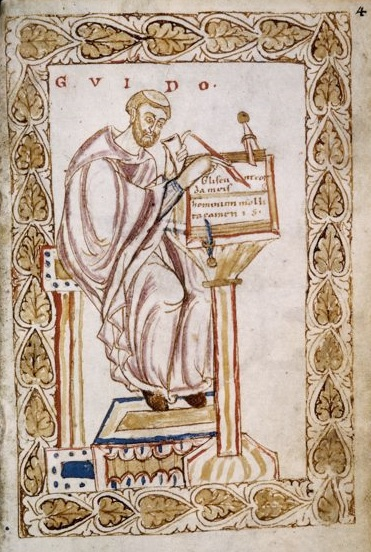
\includegraphics[height=.5\textheight]{img/Guido_van_Arezzo.jpg}}
	
	\begin{itemize}
		\item Mönch, Musiktheoretiker und Lehrer 
		\item Erfinder der Solmisation (Technik der Gesangslehre)\\
		~~~\conclude~\enquote{do re mi fa so la si do}\\
		%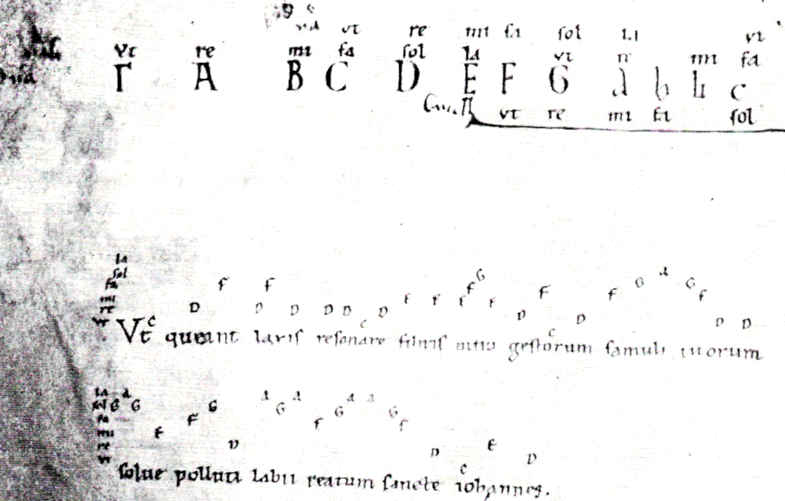
\includegraphics[height=.3\textheight]{img/Guido_van_Arezzo__Ut_queant_laxis.png}
	\end{itemize}
	
	\begin{infobox}[.75\textwidth]{Übung für Arezzos Schüler}
		Mithilfe einer Abbildung, die jedem Vokal aus $\{a,e,i,o,u\}$\\Noten einer Skala (z.B. C D E F G) zuweist,\\kann ein beliebiger Text \enquote{vertont} werden.
	\end{infobox}

	\medskip
	\conclude~erster Musikalgorithmus der Geschichte (ein sogenanntes \textbf{Translational Model})

	\medskip
	\hfill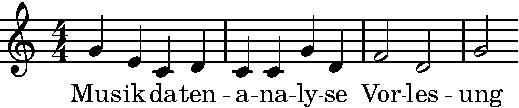
\includegraphics[height=1.5cm]{lily/Arezzo.pdf}\audioplayer{lily/Arezzo.midi}
\end{frame}

\begin{frame}{Geschichte ohne Computer}{Musikalisches Würfelspiel}

	\begin{itemize}
	\item Erfinder: Johann\,P. Kirnberger, 1757 \conclude~beliebter Zeitvertreib bis Ende 18.\,Jh.
	\item Berühmter Vertreter: Wolfgang A. \textbf{Mozarts} (1793) \citep[294d/516f]{KoechelVZ}\\
	~~~\enquote{Anleitung zum \textbf{Componieren von Walzern} vermittels zweier \textbf{Würfel}} 
	\end{itemize}	
	
	\begin{multicols}{2}
	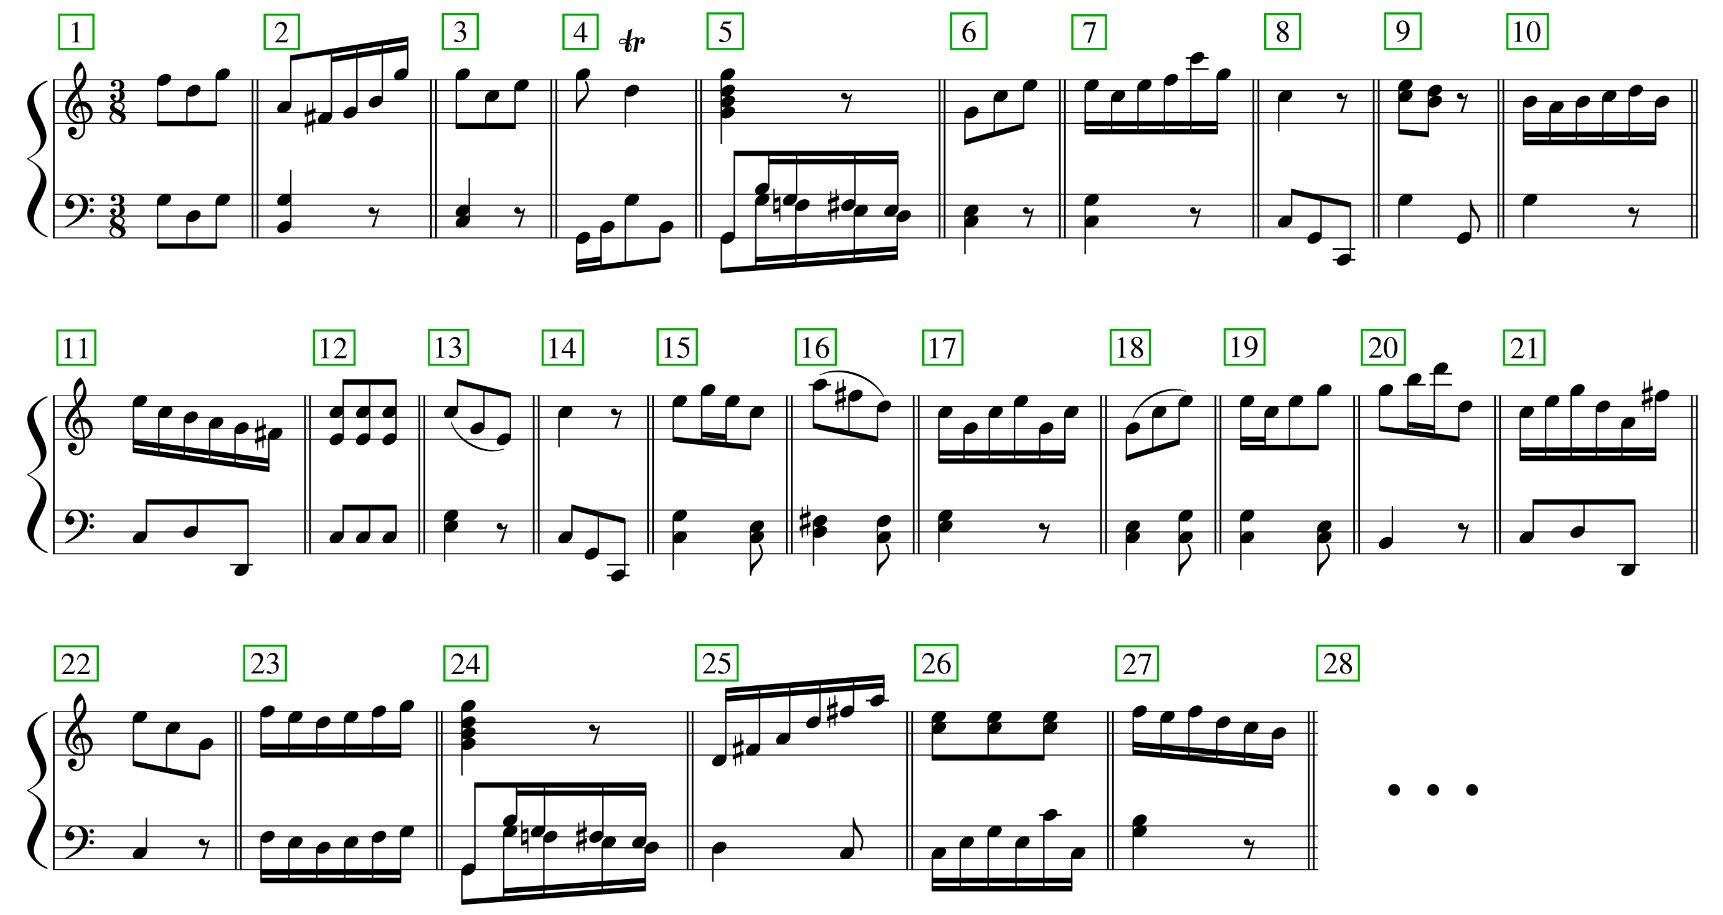
\includegraphics[width=.52\textwidth]{img/Wuerfelspiel_Noten.png}
	
	~~\resizebox{.45\textwidth}{!}{
		\csvreader[tabular=|r|rrrrrr|,
		table head=\toprule,
		table foot=\bottomrule,
		no head,
		late after line=\\,
		late after first line=\\\midrule,]{img/Wuerfelspiel_Zahlentafel.csv}{}{
			\csvcoli & \csvcolii & \csvcoliii & \csvcoliv & \csvcolv
			%& \csvcolvi & \csvcolvii & \csvcolviii
			& \large{$\boldsymbol{\cdots}$} & \csvcolxvii
		}
	}
	\end{multicols}

	\hfill \footnotesize Digitalisierte Version: \href{https://www.buschs.de/Mozart/Mozart.html}{\texttt{buschs.de/Mozart/Mozart.html}}
	
\end{frame}

\begin{frame}{Geschichte ohne Computer}{Serielle Musik}
	\begin{itemize}
		\item Ab etwa 1948: Generalisierung der \emph{Zwölftontechnik} (1920)\\
		\hfill {\footnotesize von Arnold Schönberg (1874--1951)}
		\item Zweck: Befreiung von Redundanz, Beliebigkeit und persönlichem Geschmack
		\item Nicht nur Tonhöhe, sondern auch Tondauer, Lautstärke, Artikulation und Klangfarbe werden nach festgelegten \emph{Reihen} bestimmt
		
		\bigskip
		\underline{Primitives Beispiel:}\\
		\medskip
		
		\mbox{
			\hspace{-1cm}
			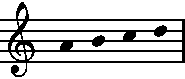
\includegraphics[height=1cm]{lily/SerielleMusik_pitches.pdf}
			~\raisebox{.3cm}{$\Large\boldsymbol{*}$}
			~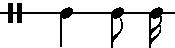
\includegraphics[height=.6cm]{lily/SerielleMusik_rhythms.pdf}
			~\raisebox{.3cm}{$\Large\boldsymbol{=}$}
			~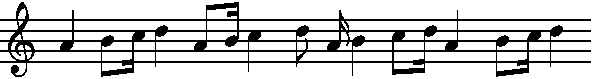
\includegraphics[height=1cm]{lily/SerielleMusik_folded_nobars.pdf}
		}
	
		\bigskip
		\hfill \raisebox{.3cm}{Einbetten in 4/4-Takt:}
		~~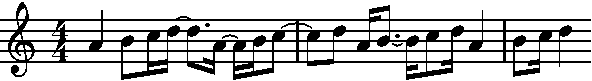
\includegraphics[height=1cm]{lily/SerielleMusik_folded.pdf}
		\audioplayer{lily/SerielleMusik_folded.midi}
	\end{itemize}

\end{frame}

\begin{frame}{Geschichte ohne Computer}{Serielle Musik II}
	
	\vspace{-.8cm}
	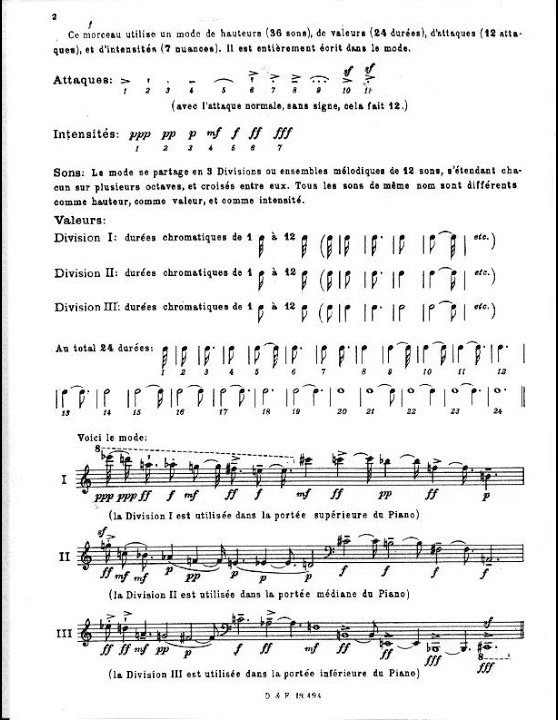
\includegraphics[width=.32\textwidth]{img/Olivier_Messiaen_Regeln.jpg}
	\hfill\raisebox{2.5cm}{\Huge\Conclude}~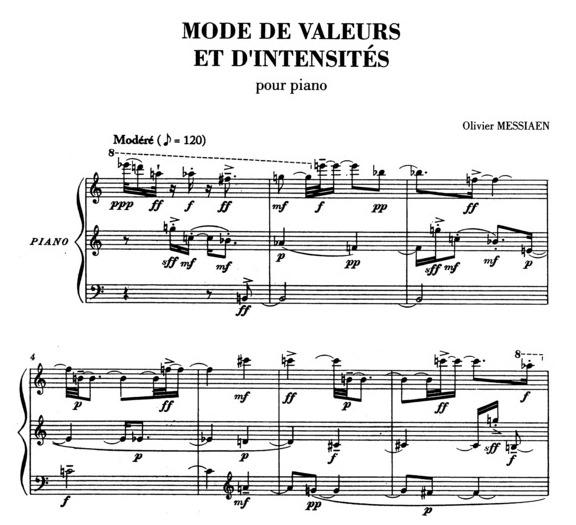
\includegraphics[width=.44\textwidth]{img/Olivier_Messiaen_Score.png}\audioplayer{audio/Olivier_Messiaen-Mode_de_valeurs_et_d_intensites.mp4}~~
	
	\begin{itemize}
		\item[\conclude] (Sehr) strenge Regeln $\hat=$ Handlungsvorschriften (Algorithmen)
		\item[\Conclude] Rezeption: komplexe Strukturen sind bei Höreindruck nicht mehr fassbar\\
		\hfill {\small (ein Problem, das die automatische Komposition erbt!)}
	\end{itemize}
	
	%Empfehlung: Olivier Messiaen: \emph{Mode de valeurs et d'intensités} (1949) \url{youtube.com/watch?v=tG9TAqBZa4}
\end{frame}

%\begin{frame}{Geschichte ohne Computer}{Serielle Musik}
%TODO
%	\todobox{Zeige Babbitt Square, um zu zeigen -> haben es sehr weit getrieben\\
%	Mathe darunter?}
%\end{frame}

\begin{frame}{Geschichte mit Computer}{Iannis Xenakis (1922--2001) -- \emph{Stochastische} Musik}
	
	Xenakis untersucht bestehende mathematische Modelle\\
	~~~~~\conclude~Komplexität überschreitet später \textbf{manuelle \enquote{Ausrechenbarkeit}}\\
	\medskip
	
	\enquote{Achorripsis} (1957) basiert auf der Poisson-Verteilung $P_\lambda(k) = \frac{\lambda^k}{k!}e^{-k}$
	
	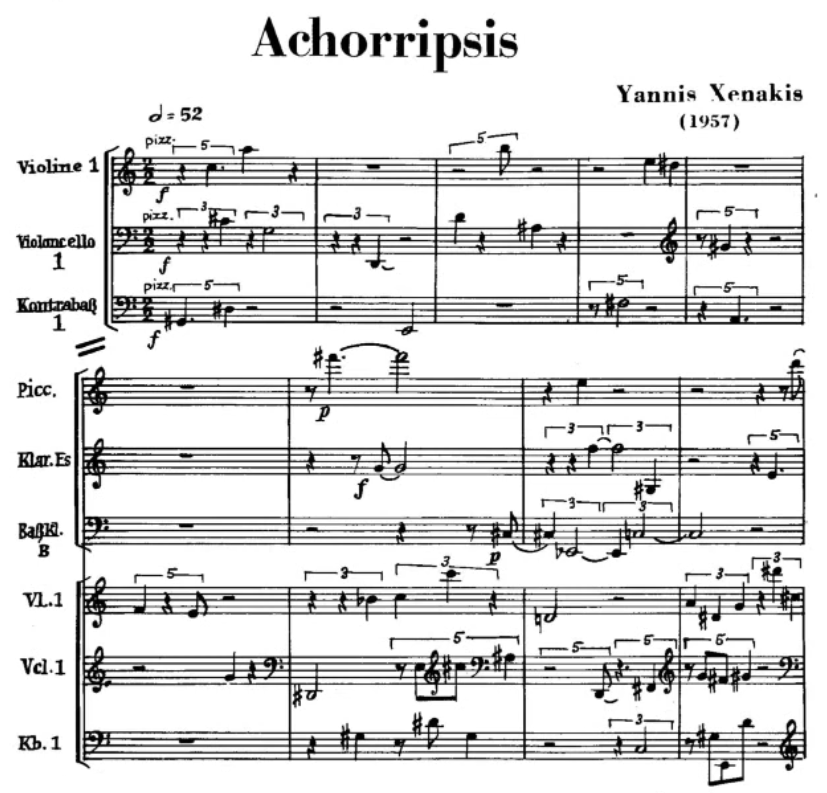
\includegraphics[width=.33\textwidth]{img/Achorripsis_Noten.png}
	~~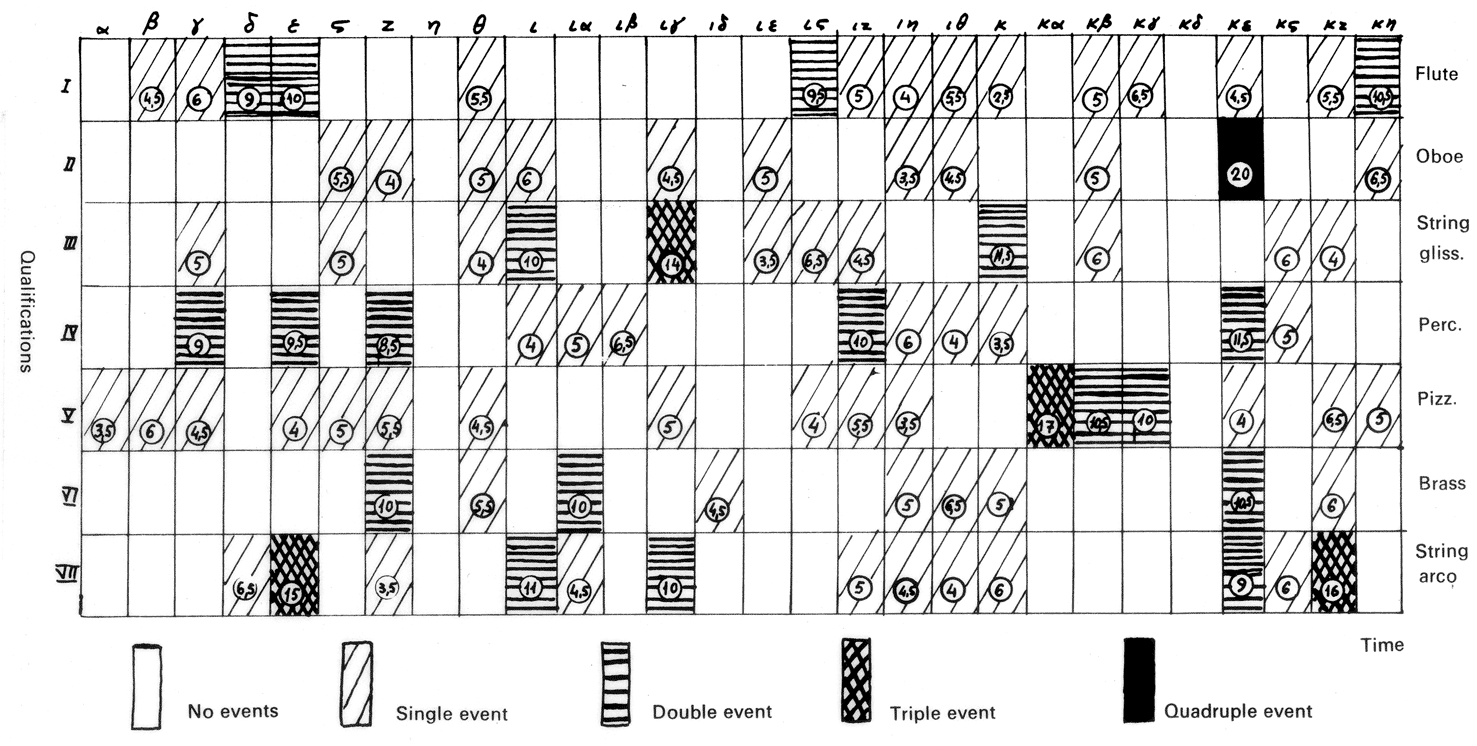
\includegraphics[width=.6\textwidth]{img/Achorripsis_CellMatrix_from_FormalizedMusic.png}
	
	
	%Erklärung und Literaturverweise: second.wiki/wiki/achorripsis
	%Score: youtube.com/watch?v=rEyqJPW3Hi8
	%Visualisierung: youtube.com/watch?v=WasFTDq0dJI
\end{frame}

\begin{frame}{Geschichte mit Computer}{Illiac Suite (String Quartet No. 4)}
	
	\drawat{11.5cm,1.5cm}{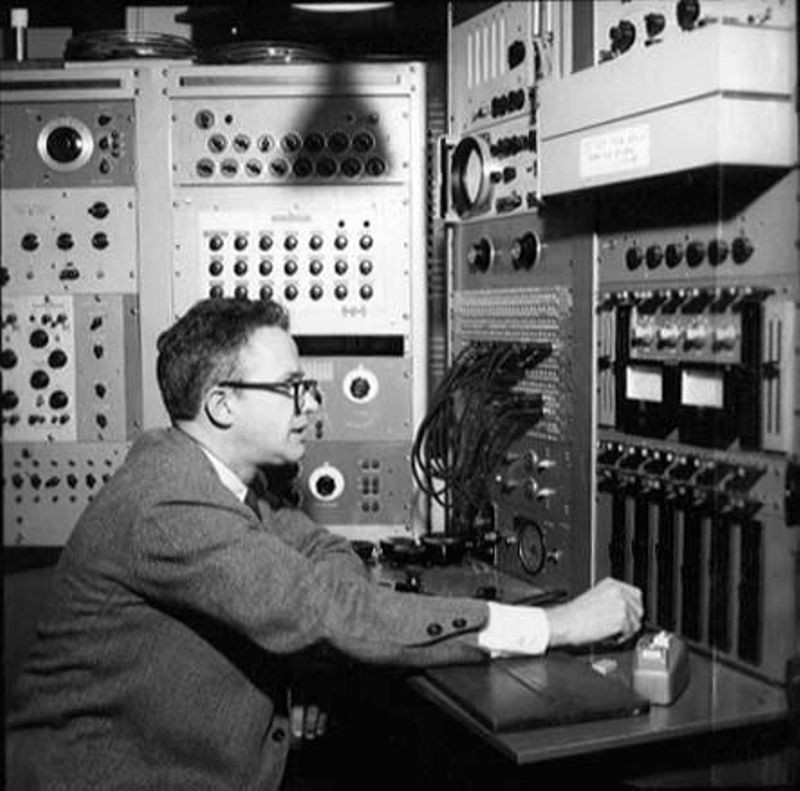
\includegraphics[width=3.5cm]{img/hiller.jpg}}
	
	\begin{itemize}
		\item Gilt als \enquote{erster echter Versuch}
		\item 4 Sätze:
		\begin{enumerate}
			\item \emph{cantus firmi}
			\item Vierstimmiger Satz mit Kompositionsregeln
			\item Experiment mit Rhythmus, Dynamik und Artikulation \audioplayer{audio/Lejaren_Hiller_-_Illiac_Suite_for_String_Quartet_3of4.mp3}
			\item Einfache stochastische Modelle
		\end{enumerate}
	\end{itemize}
	
	\bigskip
	\attentionSign~Aufführung mit menschlichen Musikern (Streichquartett)

	
\end{frame}

\begin{frame}{Geschichte mit Computer}{Band-In-A-Box (1990)}
	\centering
	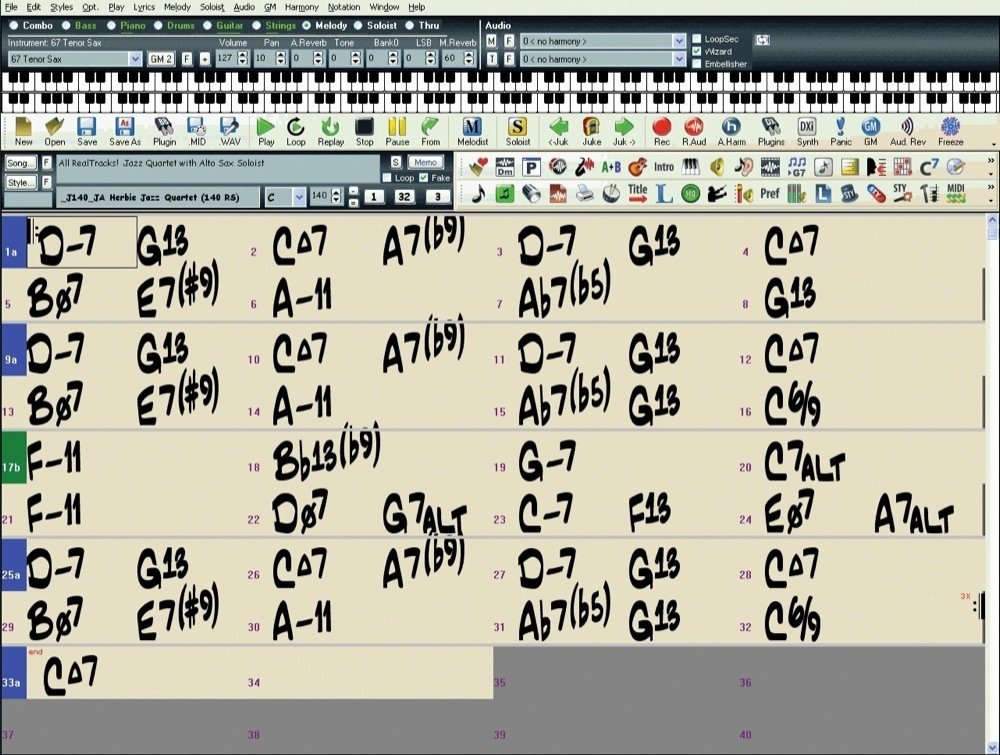
\includegraphics[width=.6\textwidth]{img/bandinabox.jpg}
	\parbox{0.3\textwidth}{
		\begin{itemize}
			\vspace{-2cm}
			\item öffentliche Aufmerksamkeit
			\item kommerzieller Durchbruch
		\end{itemize}
	}
\end{frame}


%%%%%%%%%%%%%%%%%%%%%%%%%%%%%%%%%%%%%%%%%%%%%%%%%%%%%%
%%%%%%%%%%%%%%%%%%%%%%%%%%%%%%%%%%%%%%%%%%%%%%%%%%%%%%
\section{Vorschläge zur Kategorisierung und Beispiele}
\newcommand{\dimOneTitle}{Automatisch vs. algorithmisch}
\newcommand{\dimTwoTitle}{Deterministisch vs. stochastisch}
\newcommand{\dimThreeTitle}{Regelbasiert vs. datenbasiert}
\newcommand{\dimFourTitle}{Ausgabe: Scores vs. Sounds}
\newcommand{\dimFiveTitle}{Zielsetzung/Aufwand/Anspruch}
\newcommand{\dimSixTitle}{Statisch/autonom/aleatorisch vs. adaptiv/interaktiv/echtzeitfähig/human-in-the-loop}

\begin{frame}[t]{Vorschläge zur Kategorisierung}
	\vspace{-.5cm}
	\begin{center}
		In der Literatur (bisher) keine Einigkeit.
	\end{center}
	%\medskip
	
	Vorschläge:
	\begin{itemize}
		\item[\textbf{I.}] \dimOneTitle 
		\item[\textbf{II.}] \dimTwoTitle
		\item[\textbf{III.}] \dimThreeTitle
		\item[\textbf{IV.}] \dimFourTitle
		\item[\textbf{V.}] \dimFiveTitle
		\item[\textbf{VI.}] \dimSixTitle
	\end{itemize}
	\medskip
	
	\begin{itemize}
		\item[\warnSign] Diese \enquote{Dimensionen} sind nicht orthogonal.
		\item[\warnSign] Die Aufzählung bietet keine Vollständigkeit.
	\end{itemize}
\end{frame}

\begin{frame}{II. \dimTwoTitle}{Lindenmayer-System (deterministisch)}
	Ein L-System ist ein Quadrupel $G=(V,S,\omega,P)$, wobei
	\begin{itemize}
		\item $V$ eine Menge an (ersetzbaren) \textbf{Variablen},
		\item $S$ ein Menge an (unersetzbaren) Zeichen,
		\item $\omega$ ein Startwort (Axiom) und
		\item $P$ eine Menge an \textbf{Produktionsregeln} darstellen.
	\end{itemize}

	\begin{multicols}{2}
		\underline{Ein Beispiel}:\\
		\begin{itemize}
			\item[] Sei $V = \{a,b\},~S=\emptyset,~\omega=a$.
			\item[] $P$ bestehe aus
			\item[] ~~~$a \mapsto b$
			\item[] ~~~$b \mapsto ab$
		\end{itemize}
	\columnbreak

		\begin{itemize}
			\footnotesize
			\item[n=0:] a
			\item[n=1:] b
			\item[n=2:] ab
			\item[n=3:] bab
			\item[n=4:] abbab
			\item[n=5:] bababbab
			\item[\dots] usw.
		\end{itemize}
	\end{multicols}

	\drawat{11.5cm,4.7cm}{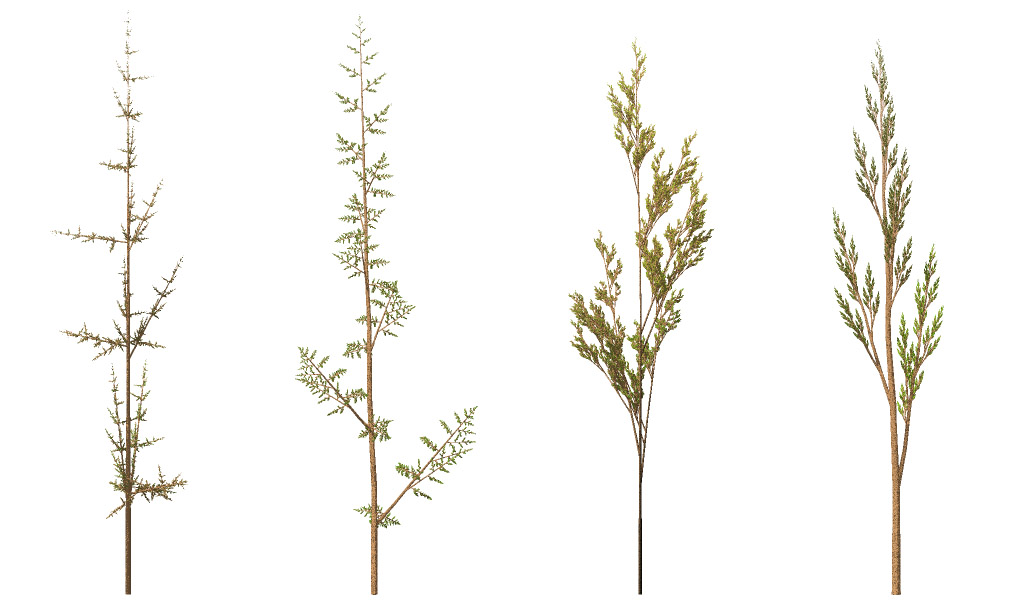
\includegraphics[height=.4\textheight]{img/Fractal_weeds.jpg}}
\end{frame}

\begin{frame}{II. \dimTwoTitle}{Lindenmayer-System II}
	\parbox{.25\textwidth}{
		\begin{itemize}
			\scriptsize
			\item[n=0:] a
			\item[n=1:] b
			\item[n=2:] ab
			\item[n=3:] bab
			\item[n=4:] abbab
			\item[n=5:] \fbox{bababbab}
			\item[\dots] usw.
		\end{itemize}
	}
	\parbox{.6\textwidth}{
		\raisebox{.5cm}{(1)~\audioplayer{lily/LSystem_1.midi}}~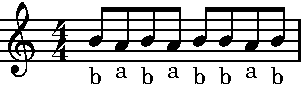
\includegraphics[height=1.3cm]{lily/LSystem_1.pdf}
		
		\medskip
		\raisebox{.7cm}{(2)~\audioplayer{lily/LSystem_2.midi}}~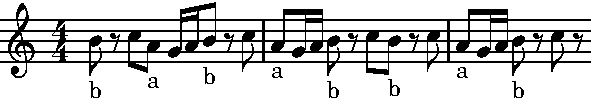
\includegraphics[height=1.5cm]{lily/LSystem_2.pdf}
		
		\medskip
		\raisebox{.7cm}{(3)~\audioplayer{lily/LSystem_3.midi}}~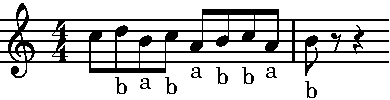
\includegraphics[height=1.5cm]{lily/LSystem_3.pdf}
	}

	\bigskip
	\hrule
	\bigskip
	Determinismus simuliert den menschlichen Kompositionsprozess niemals akkurat\\
	\hfill\conclude~es fehlen Zufallsprozesse wie Intuition und \enquote{glückliche Fehler}
\end{frame}

\begin{frame}{II. \dimTwoTitle}{Fraktale (deterministisch)}
	\drawat{2cm,3cm}{\parbox{3cm}{Romanesco\\(Blumenkohl)}}
	\begin{center}
		~~~~~~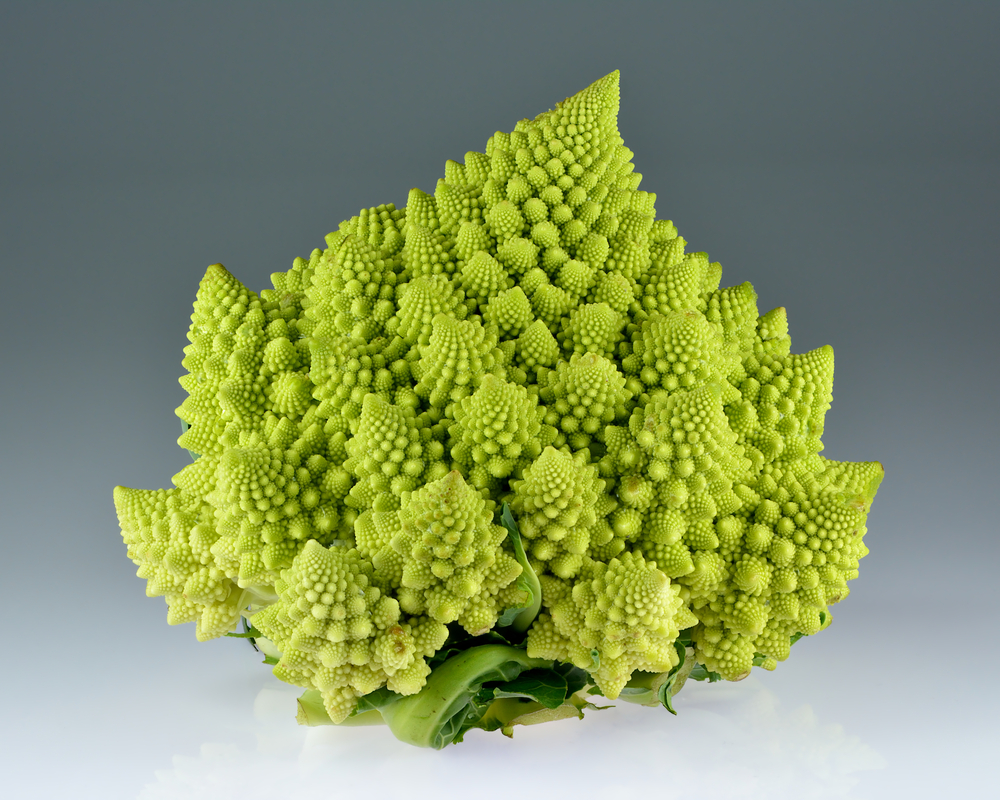
\includegraphics[width=.46\textwidth]{img/Romanesco_broccoli.jpg}
	\end{center}
	\hfill\small \underline{Empfehlung}: Gary Lee Nelson -- \enquote{Fractal Mountains} (1992)\\
	\hfill\conclude~96 Tonschritte pro Oktave\\
	\hfill\tiny\url{youtube.com/watch?v=KV3V3c8mqGs}\\
	\hfill\url{timara.oberlin.edu/gnelson/PapersPDF/GNfract.pdf}

\end{frame}

\begin{frame}{II. \dimTwoTitle}{Markov-Kette (stochastisch)}
	Eine Markov-Kette ist ein \emph{stochastischer Prozess}
	\begin{center}
		{$=$ math. Beschreibung von zeitl. geord., zufälligen Vorgängen} (z.B. Börsenkurs)
	\end{center}

	\underline{Markov-Eigenschaft}:
	\begin{center}
		$P(X_{t+1} = s_{j_{t+1}} | X_t = s_{j_t}, X_{t-1} = s_{j_{t-1}},\dots,X_{0} = s_{j_0}) = P(X_{t+1} = s_{j_{t+1}} | X_t = s_{j_t})$
	\end{center}

	\conclude~Folgezustand hängt \underline{nur} vom aktuellen Zustand ab (\enquote{Gedächtnislosigkeit})

\end{frame}

\begin{frame}{II. \dimTwoTitle}{Markov-Kette (Beispiel 1)}
	
	\parbox{.6\textwidth}{
		\centering
		\underline{Hänschen Klein}
		\fbox{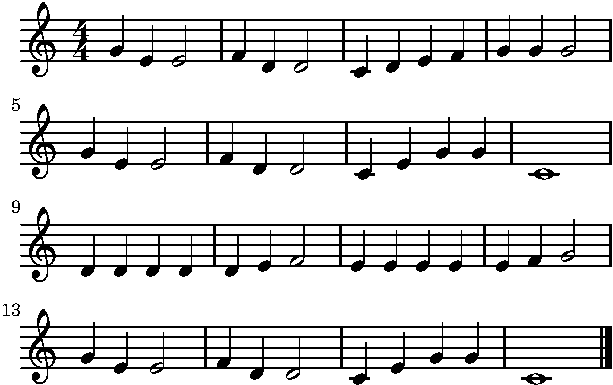
\includegraphics[width=.5\textwidth]{lily/HaenschenKlein.pdf}}
	}
	\parbox{.39\textwidth}{
		48 Noten\\
		6x C, 12x D, 15x E, 6x F, 11x G\\
		
		\begin{itemize}
			\item $P(X=C) = \frac{6}{48} = 12.5\%$
			\item $P(X=D) = \frac{12}{48} = 25.0\%$
			\item $P(X=E) = \frac{15}{48} = 31.25\%$
			\item $P(X=F) = \frac{6}{48} = 12.5\%$
			\item $P(X=G) = \frac{11}{48} = 22.92\%$
		\end{itemize}
	}

	\hfill \Conclude~\raisebox{-.25cm}{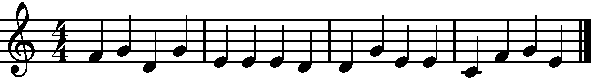
\includegraphics[height=.8cm]{lily/HaenschenKlein_random.pdf}}\,\audioplayer{lily/HaenschenKlein_random.midi}
	
	\medskip
	\hfill \warnSign~Noch ohne Vorbedingung
	
	% 6x c, 12x d, 15x e, 6x f, 11x g
\end{frame}

\begin{frame}{II. \dimTwoTitle}{Markov-Kette (Beispiel 2)}
	
	\mbox{
		\parbox{.54\textwidth}{
			\centering
			\underline{Hänschen Klein}
			\fbox{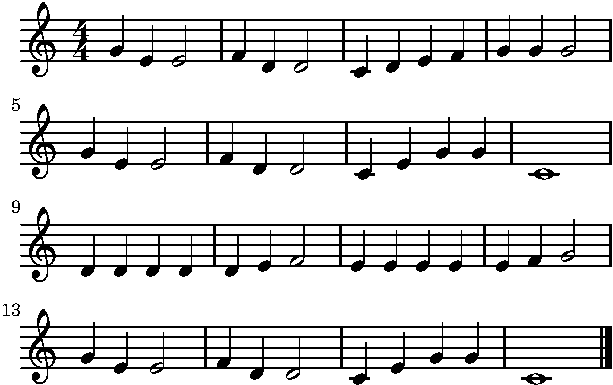
\includegraphics[width=.5\textwidth]{lily/HaenschenKlein.pdf}}
		}
		\parbox{.5\textwidth}{
			Markov-Eigenschaft:
			
			\begin{itemize}
				\item $P(X_{t+1} = C | X_{t} = C) = 0$
				\item[] ~~$\vdots$
				\item $P(X_{t+1} = G | X_{t} = G) = \frac{6}{47} \small= 12.77\%$
				\item[] ~~$\vdots$
				\item $P(X_{t+1} = E | X_{t} = G) = \frac{3}{47} \small= 6.38\%$
			\end{itemize}
		}
	}

	\medskip
	\hspace{4.5cm}\underline{Erweiterung} möglich, z.B. relative Intervalle, Rhythmus, ...\\
	\smallskip
	\hspace{4.5cm}\underline{Lernverfahren}: \emph{Hidden Markov Model}
\end{frame}

\begin{frame}{III. \dimThreeTitle}{Kemal Ebcio\u{g}lu: CHORAL Project (regelbasiert)}
	\textbf{Expertensysteme} (auch \enquote{wissenbasiertes} System) implementieren erkannt/bekannte Regeln als (logisches) Programm.
	\medskip
	
	\vspace{-.5cm}
	\mbox{\underline{Beispielaufgabe}: 4-stimmige Harmonisierung im Stile J.\,S.\,Bachs. \raisebox{-.5cm}{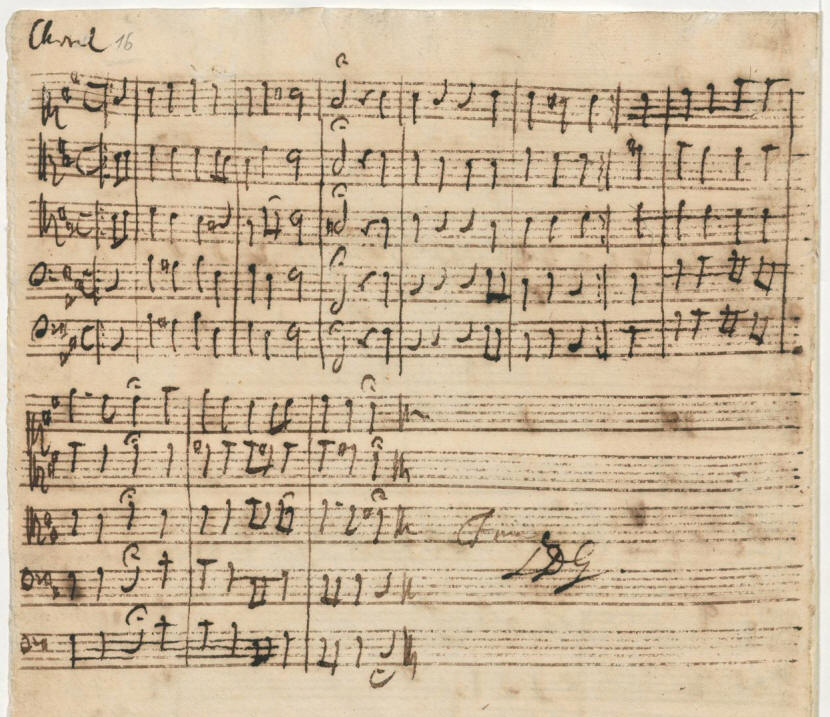
\includegraphics[height=1.5cm, clip, trim=0cm 20cm 0cm 3cm]{img/bwv84_choral_autograph.png}}}
	\medskip
	
	\begin{quote}
	\enquote{The rules and \textbf{heuristics} were found mainly from empirical observation of the
		chorales and personal intuitions, although we used a number of \textbf{traditional treatise}} {\footnotesize\citep[S.73]{CHORAL_report}}\\
	\end{quote}
	{\color{TUDoGreen}\textbf{Def.}} \emph{Heuristik}: Handslungsvorschrift, deren Korrektheit auf Empirie oder Intuition fußt und deren Ergebnis nicht unbedingt optimal ist.
	\medskip
	
	Regeln in klassischen Kompositionslehren sind typischerweise Heuristiken, da sie nie ausnahmslos gelten (z.B. \emph{Quintparallelverbot}).
\end{frame}
\begin{frame}[t]{III. \dimThreeTitle}{CHORAL Project (1986): 350 Regeln (\warnSign)}
	\parbox{.7\textwidth}{
		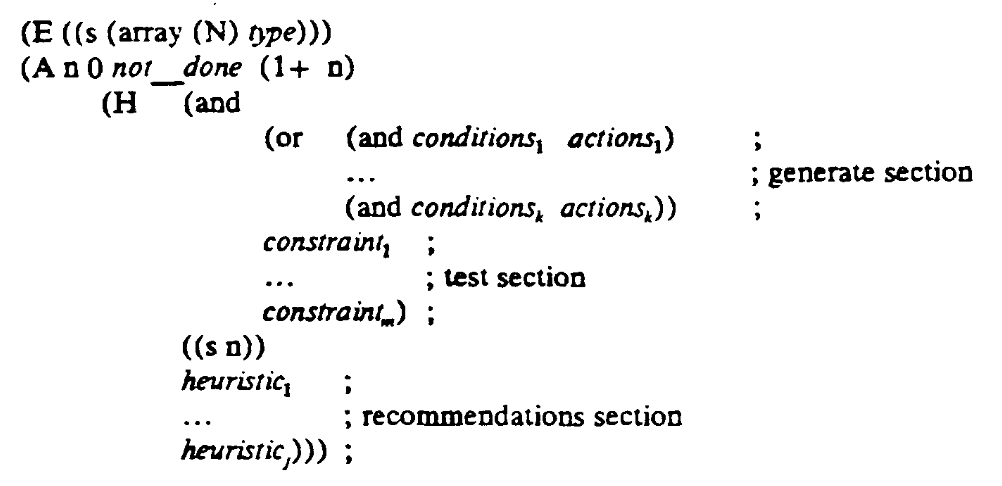
\includegraphics[width=.7\textwidth]{img/CHORAL_loop.png}
	}
	
	\drawat{8.5cm,4cm}{
		\begin{infobox}[6.5cm]{Regelbeispiel \only<1>{1}\only<2>{2}\only<3>{3}\only<4>{4}}
			\only<1>{
				In the very first chord, one can start with either in the tonic (I) \textbf{or} the dominant(V) degree of the key. \citep[S.240]{CHORAL_report}
			}
			\only<2>{
				A pitch \textbf{cannot} occur both altered \textbf{and} unaltered in the same chord. \citep[S.238]{CHORAL_report}
			}
			\only<3>{
				\textbf{For} any voice v<soprano, the melodic span of the skeletal pitches of voice v from the beginning of the chorale up to \textbf{and} including the current pitch, \textbf{cannot} exceed a thirteenth. \citep[S.253]{CHORAL_report}
			}
			\only<4>{\scriptsize
			\textbf{If} the previous chord is the VI degree of a major key \textbf{or} the I degree of a minor key, \textbf{and} \textbf{(}the current chord is a major triad whose root is a major second below that of the previous chord, \textbf{or} the current chord is a minor triad whose root is a perfect fourth below that of the previous chord\textbf{)}, \textbf{then} a new key whose tonic is equal to the root of the current chord can be entered at degree I. \citep[S.245]{CHORAL_report}
			}
		\end{infobox}
	}
\end{frame}

\begin{frame}{III. \dimThreeTitle}{David Copes EMI (datenbasiert)}
	
	\underline{Methodik} (informell):
	\begin{itemize}	
		\item[(1)] \textbf{deconstuction} (analyze and separate into parts)
		\item[(2)] \textbf{signatures} (commonality - retain that which signifies style) 
		\item[(3)] \textbf{compatibility} (recombinancy - recombine into new works)
		\item[\warnSign] Nach wie vor: konkrete Implementierung beruht auf \emph{Heuristiken}
	\end{itemize}
	
	\medskip
	\begin{quote}
		\enquote{All the great books are constructed from recombinations of twenty-six letters. Similarly, most of the great works of Western art music exist as recombinations of twelve pitches. The secret lies \textbf{not} in the \textbf{invention of new letters} or notes but in the subtlety and \textbf{elegance} of their \textbf{recombination}.} - {\footnotesize David Cope (1996)}
		\\\hfill{\tiny(\url{artsites.ucsc.edu/faculty/cope/experiments.htm})}
	\end{quote}
	
	Datensatz beschreibt den \emph{Stil} eines Komponisten \citep{Cope96}\\
	\hfill\conclude~Alben: \enquote{Bach by Design}; \enquote{Virtual Mozart}; \enquote{Virtual Rachmaninov}
\end{frame}

\begin{frame}[t]{III. \dimThreeTitle}{Lernverfahren (datenbasiert)}
		\vspace{-1.5cm}
		\parbox{.49\textwidth}{
			\underline{Künstliches Neuron}
			\medskip

			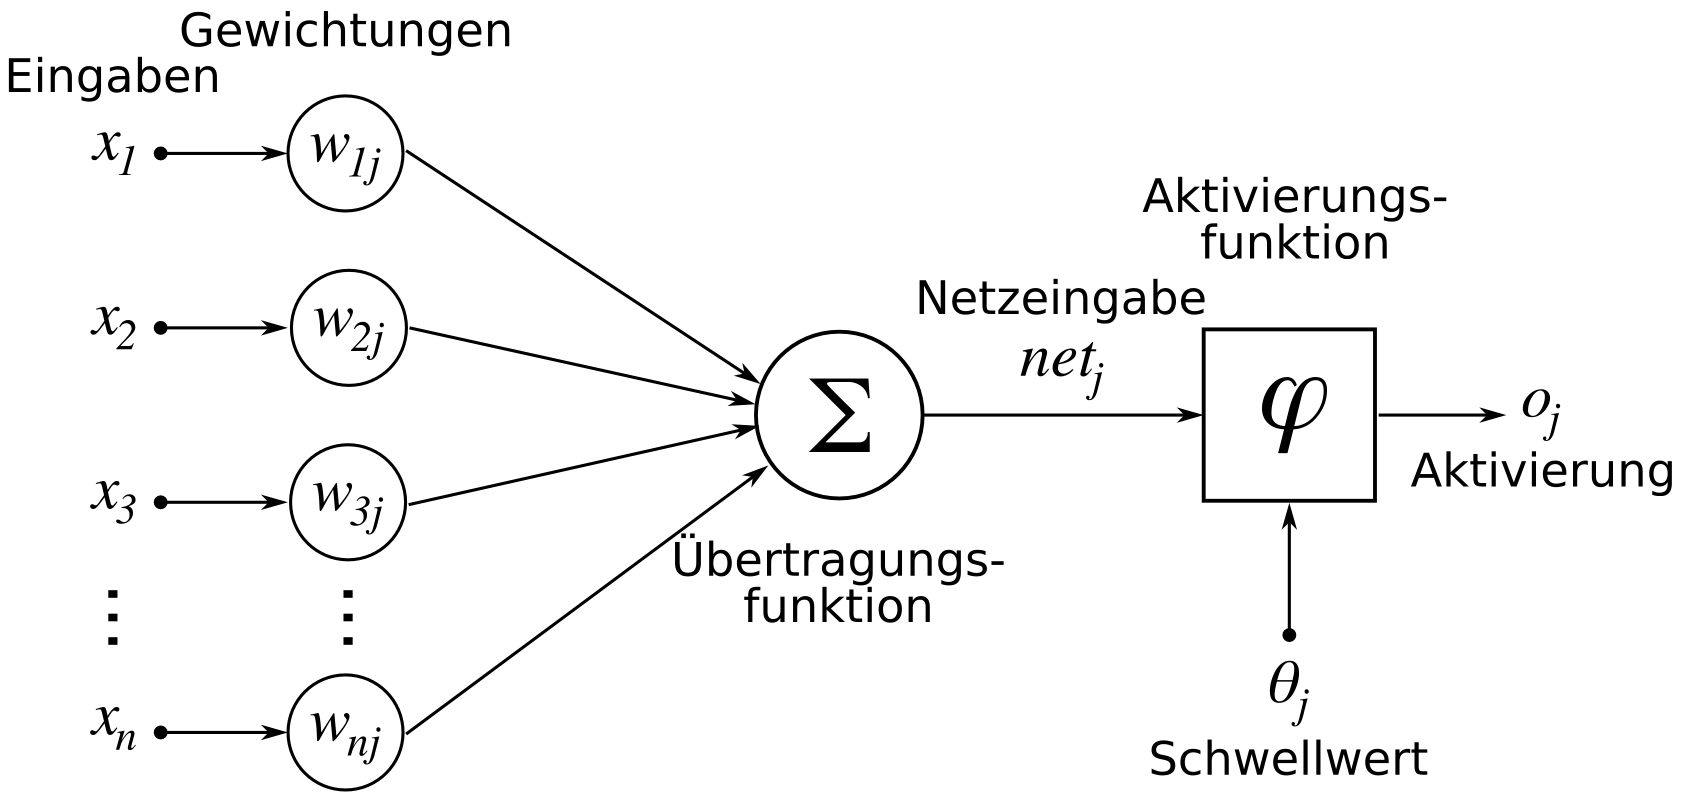
\includegraphics[width=0.49\textwidth]{img/ArtificialNeuronModel_deutsch.png}
		}
		\parbox{.49\textwidth}{
			\vspace{3cm}
			\underline{Neuronales Netz} (Mehrlagiges Perzeptron)
			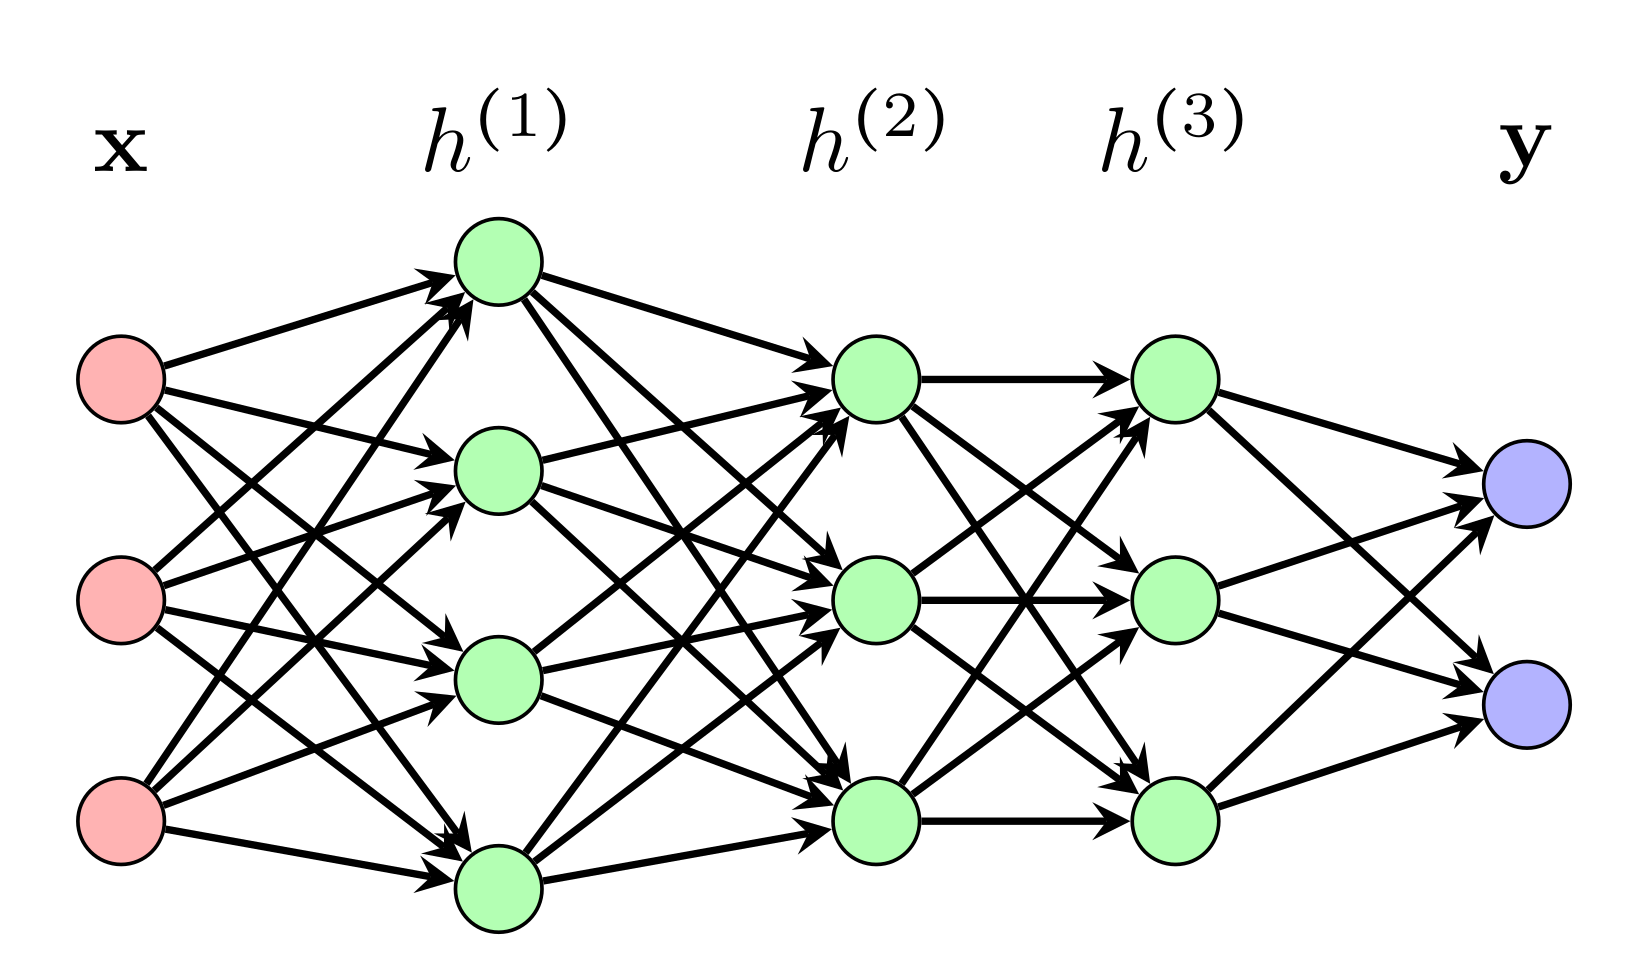
\includegraphics[width=0.49\textwidth]{img/MLP-Theorie.png}
		}
\end{frame}

\begin{frame}{IV. \dimFourTitle}
	\attentionSign~Bisher: alle Beispiele mit symbolischer Ausgabe\\
	
	\centering
	\begin{multicols}{3}
		(1) \underline{Partitur-Synthese}
		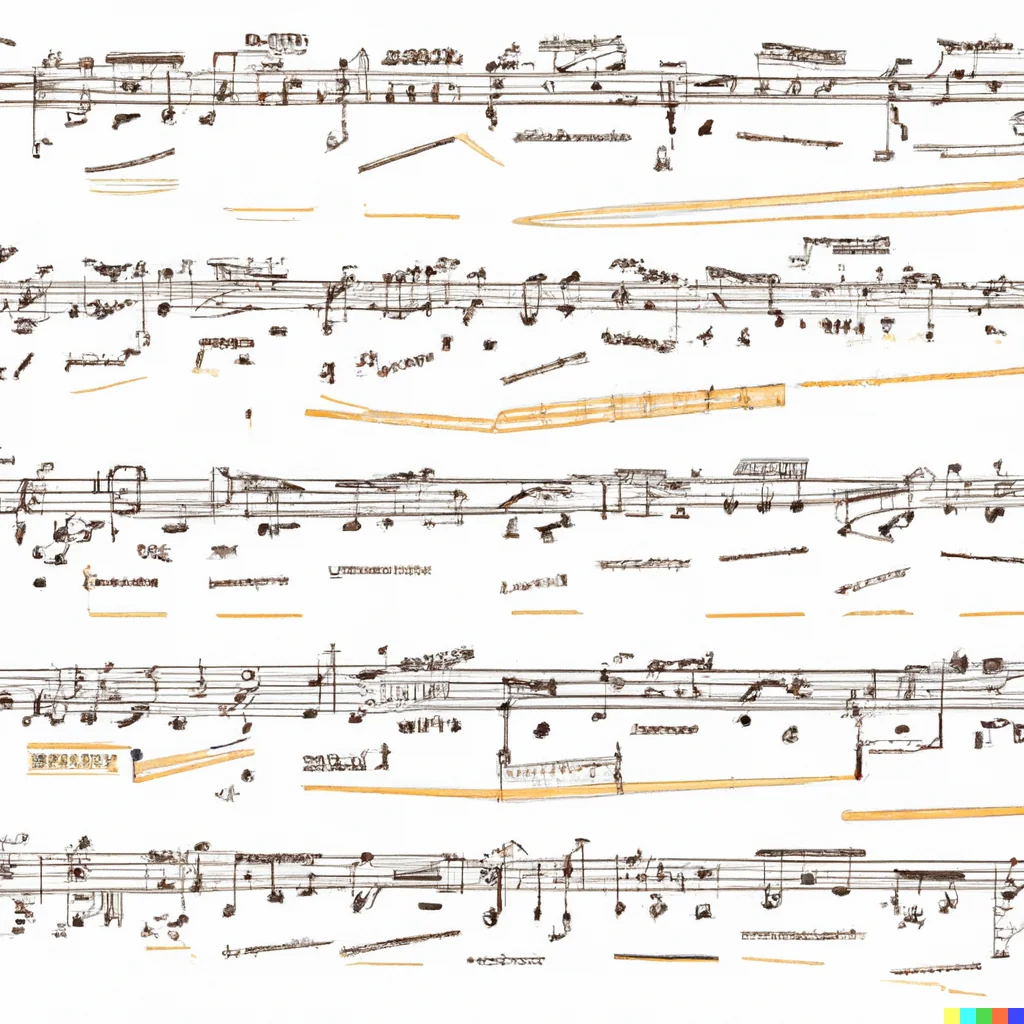
\includegraphics[width=.3\textwidth]{img/Dalle2-UndiscoveredMusicScoreByMozart.png}
		OpenAI Dall$\cdot$E\,2
	\columnbreak
	
		(2) \underline{Audio-Synthese}
		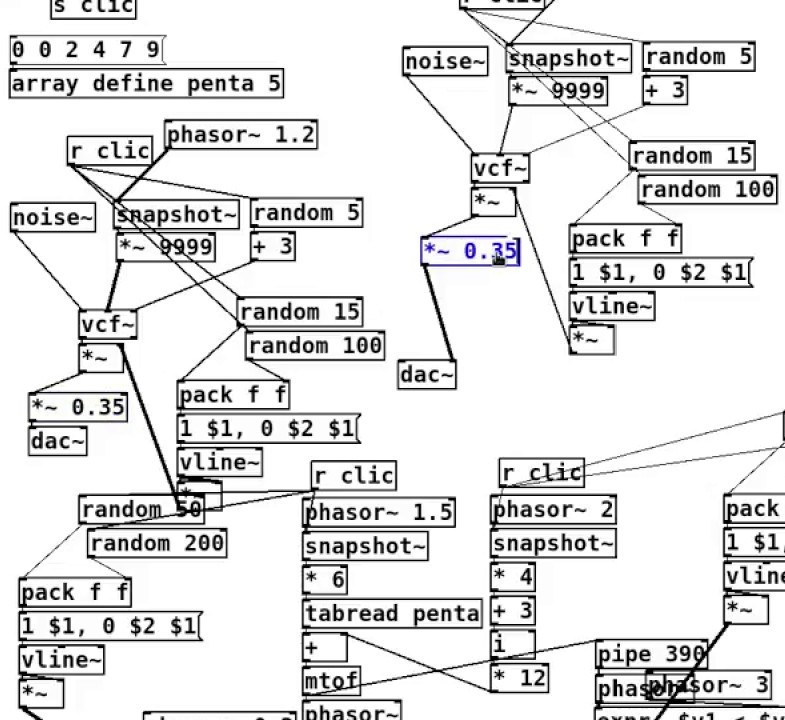
\includegraphics[width=.32\textwidth]{img/puredata.jpg}
		Pure Data (VPL)
	\columnbreak
	
		(3) \underline{Wellenform-Synthese}
		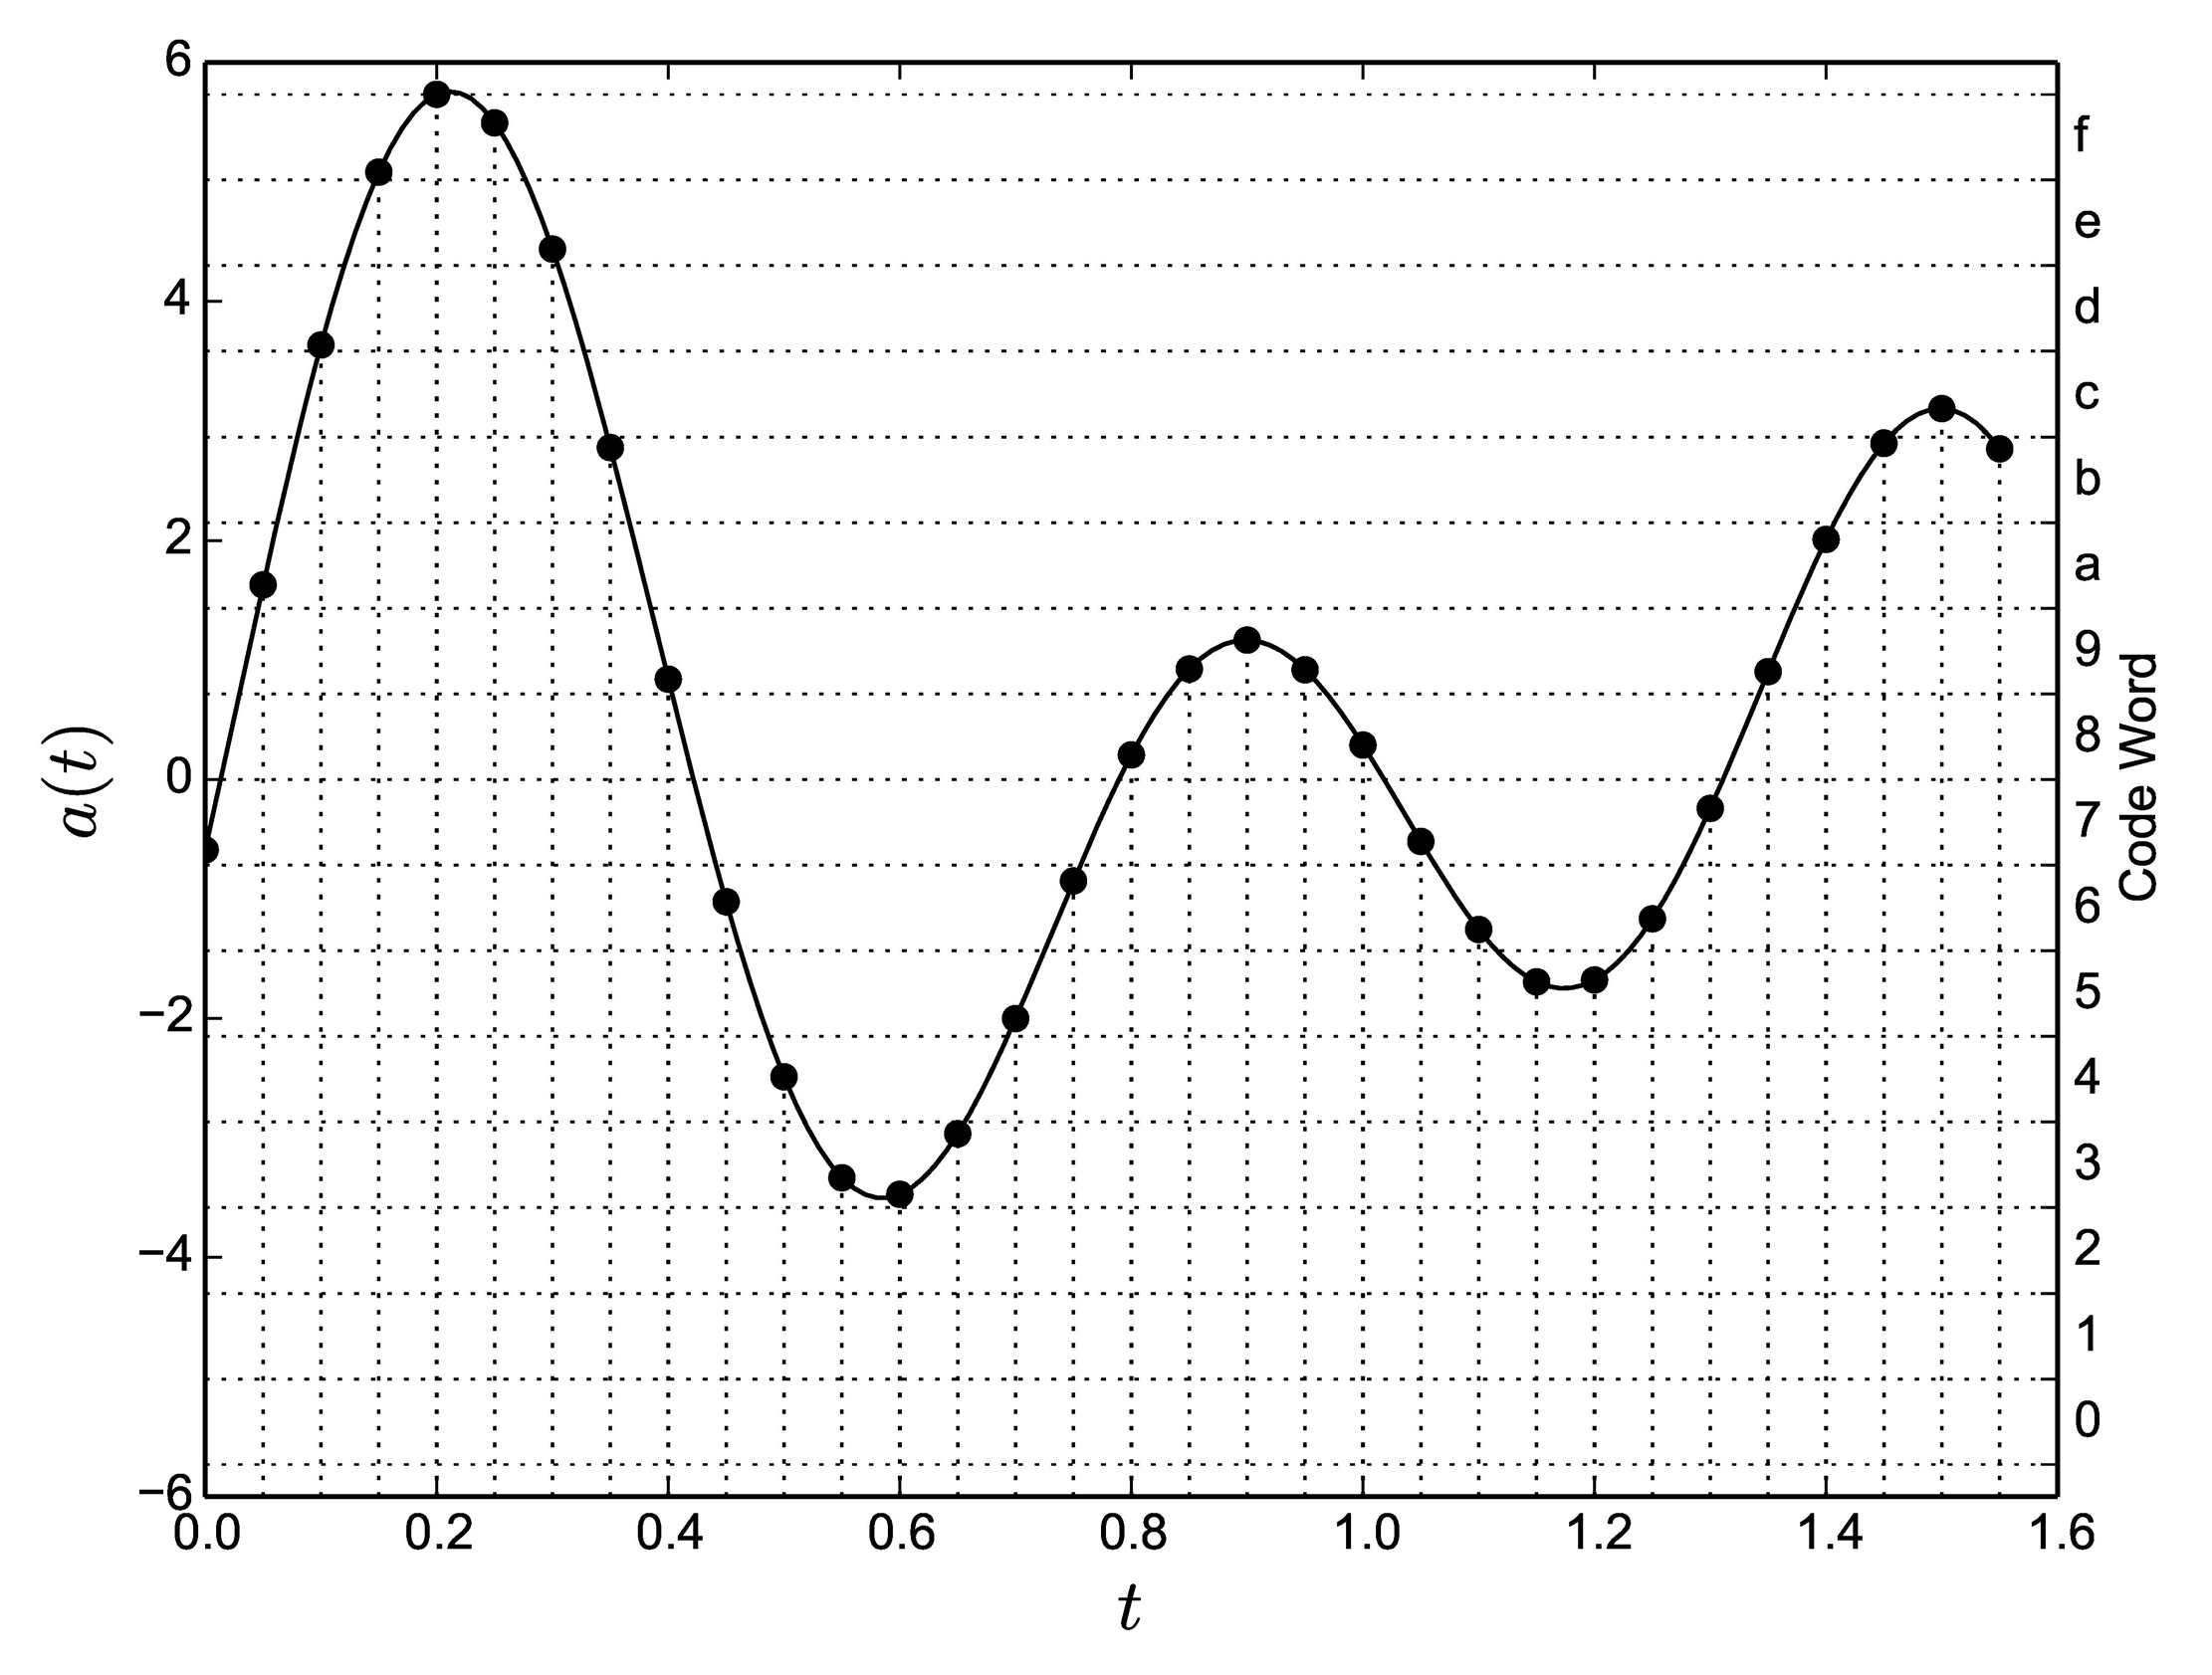
\includegraphics[width=.34\textwidth]{img/PCM_Waveform.png}
		OpenAI Jukebox\\
		
		\url{openai.com/blog/jukebox/}
	\end{multicols}
\end{frame}

\begin{frame}{V. \dimFiveTitle}{Übersicht mit Beispielen}
	\centering	
	\begin{tikzpicture}[auto]
		\draw [<->, ultra thick] (0,0) node[anchor=north west,xshift=-1cm] {\emph{beschränkt/übersichtlich}} -- (12,1) node[below] {\emph{komplex}};
		
		\node[draw] (A) at (.5,.7) {Kompositionshilfe};
		\node[draw] (B) at (3.75,1.1) {Stil-Transfer};
		\node[draw] (C) at (7.1,1.35) {Domain Competence};
		\node[draw] (D) at (11,1.6) {Original Composition};
		
		\node[above=.2cm of A] {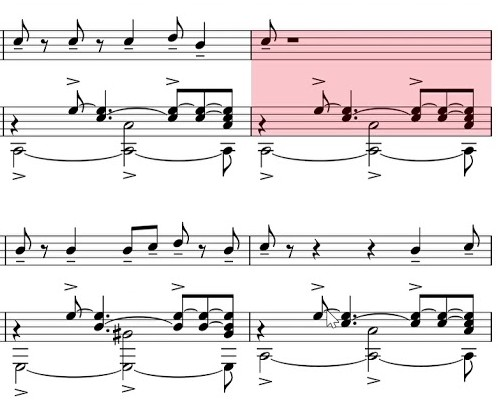
\includegraphics[width=3.2cm]{img/musescore_red.jpg}};
		\node[above=.2cm of B] {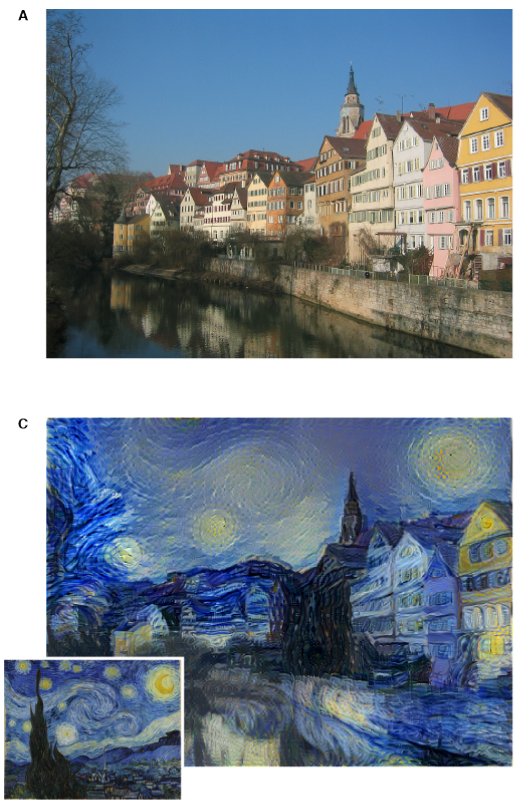
\includegraphics[width=2.6cm]{img/Stiltransfer.png}};
		\node[above=.2cm of C] {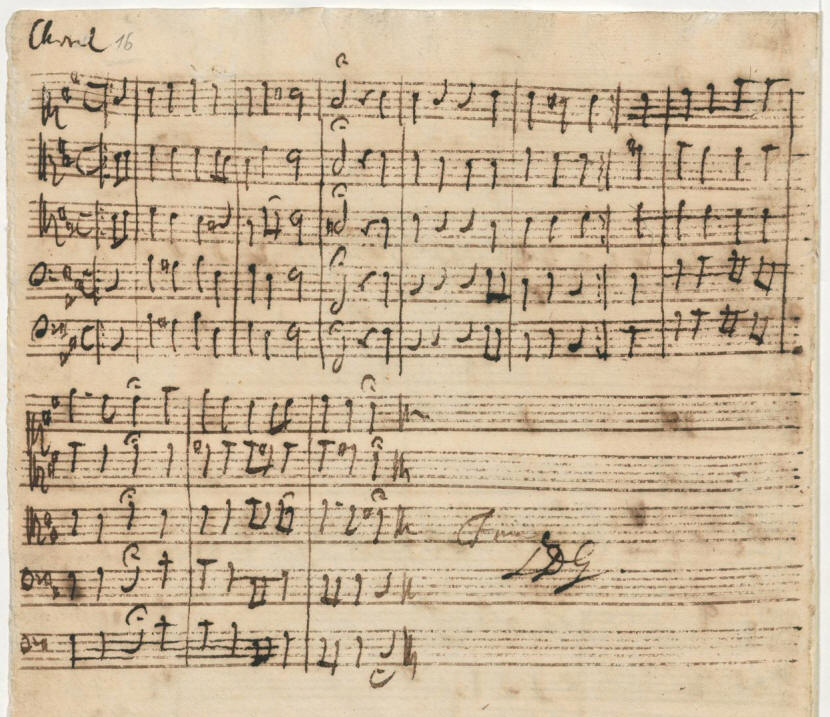
\includegraphics[width=3.5cm]{img/bwv84_choral_autograph.png}};
		\node[above=.2cm of D] {
\includegraphics[width=2.8cm]{img/blank-canvas.jpg}};
	\end{tikzpicture}
\end{frame}

\begin{frame}{V. \dimFiveTitle}{DeepBach (2017)}
	\drawat{.72\textwidth,.6cm}{
		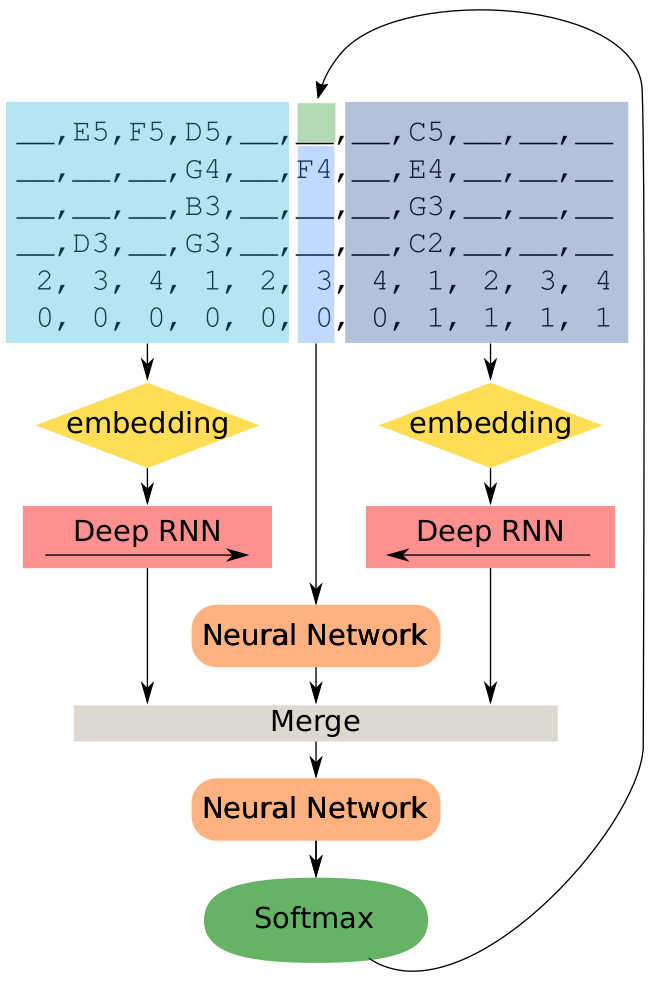
\includegraphics[height=.9\textheight]{img/DeepBach-Architektur.png}}
	\drawat{1.05\textwidth,.9\textheight}{\citep{DeepBach}}
	
	\parbox{.55\textwidth}{
		\begin{itemize}
			\item Model lernt genau einen Eintrag (Note) im 4-stimmigen Satz vorherzusagen
			\item Generierung mittels\\\medskip
			~~~~~~\underline{\emph{Pseudo-Gibbs sampling}} {\footnotesize\citep{GibbsSampling}}
			\begin{enumerate}
				\medskip
				\item Eingabe: Länge $L$, Anzahl Interationen $M$
				\item Initialisiere vierstimmiges Kompositionsraster $K$ der Länge $L$\\mit Zufallswerten
				\item Für $i=0$ bis $M$ tue:
				\begin{itemize}
					\item Wähle zufälligen Eintrag $e$ in $K$
					\item Entferne $e$
					\item Füge neue Vorhersage für $e$ ein 
				\end{itemize} 
			\end{enumerate}
		\end{itemize}
	}

	\centering
	~~~~~~~~~~~~\audioplayer{audio/DeepBach-perfectfake01.midi}
\end{frame}

\begin{frame}{V. \dimFiveTitle}{Originale Komposition: Iamus}
	\drawat{11.75cm,2.8cm}{\parbox{4cm}{\centering
		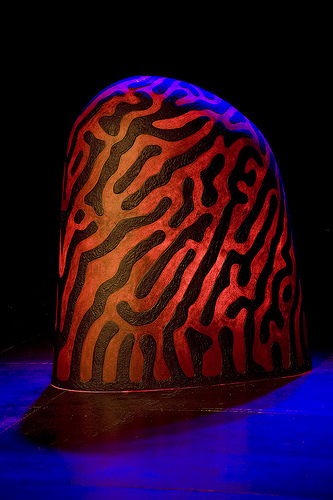
\includegraphics[width=3cm]{img/Iamus_server.jpg}
		Iamus computer cluster\\
		{\footnotesize(Universidad de Málaga)}
	}}
	
	\parbox{.8\textwidth}{
		\begin{itemize}
			\item Zielsetzung: Neue Werke zeitgenössischer klassischer Musik
			\item Stetige Fortentwicklung (Motivische Komposition) auf Grundlage eines \textbf{evolutionären Algorithmus}
			\item Veränderung folgen formellen Ästhetik-Kriterien (\emph{Formalismus})\\
			\smallskip
			~~\warnSign~Kriterien sind wieder \underline{Heuristiken}
			
			\medskip
			\item Speicherplatz: 70\,TB, Arbeitsspeicher: 704\,GB
		\end{itemize}
		
		\bigskip\bigskip
		\centering
		\enquote{Hello World} (2011) \audioplayer{audio/Iamus_Hello_World.mp3}
	}
\end{frame}

\begin{frame}{V. \dimFiveTitle}{Evolutionärer Algorithmus (EA)}
	\begin{multicols}{2}
		\hspace{-1cm}
		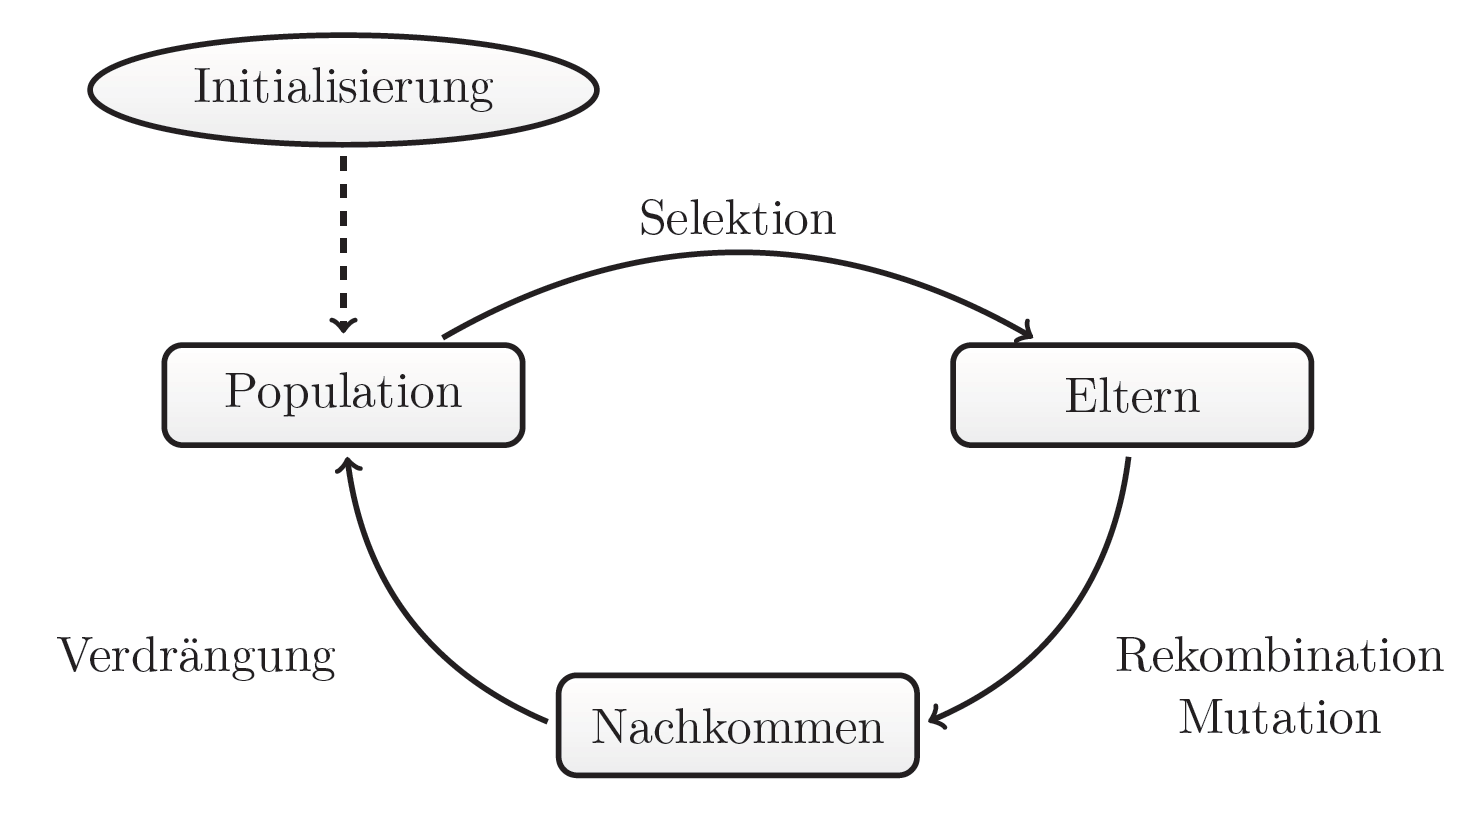
\includegraphics[width=.5\textwidth]{img/EvoAlg_Scheme.png}
		
		\columnbreak
		\begin{itemize}
			\item[Initialisierung] Zufällig oder \enquote{geschickt}
			\item[Population] enthält eine Menge an \emph{Individuen}\\
													\hfill(z.B. Melodien)
			\item[Fitness] Die Individuen werden mit einer \mbox{\emph{Fitness-Funktion} bewertet (Evaluation)}
			\item[Selektion] \enquote{Survival of the fittest}
			\item[Elternpaare] werden rekombiniert (z.B. \emph{crossover})
			\item[Mutation] Einige Individuen werden (punktuell) zufällig verändert 
			\item[Nachkommen] bilden eine nächste Generation in der Population
		\end{itemize}
	\end{multicols}
\end{frame}

\begin{frame}[t]{VI. \dimSixTitle}{Human-In-The-Loop: GenJam (1994)}
	
	Al Biles modellierte GenJam \cite{GenJam1994} als künstlichen \textbf{Musikschüler},\\
	\hfill der die Kunst der \textbf{Jazz-Improvisation} über beliebige Akkordfolgen lernt.
	
	\bigskip
	\centering
	\mbox{
		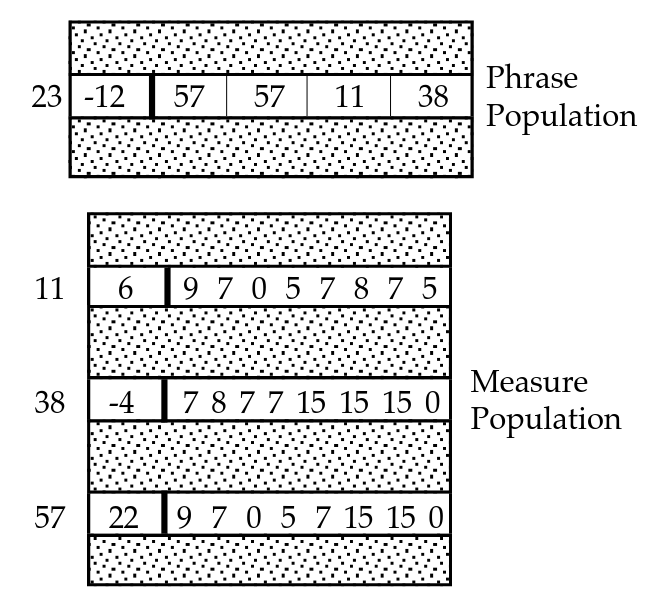
\includegraphics[width=.28\textwidth]{img/GenJam_PhraseMeasurePopulation.png}
		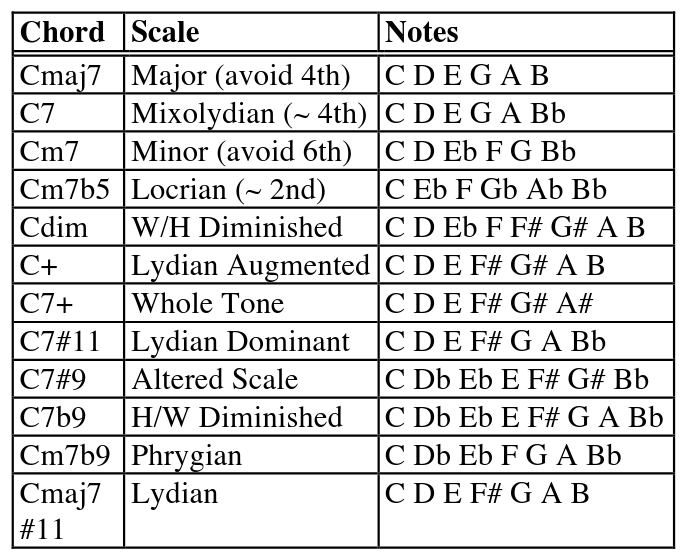
\includegraphics[width=.3\textwidth]{img/GenJam_ChordScaleMapping.png}
		~~~~~\parbox[b]{.4\textwidth}{
			\begin{itemize}
				\item[\ideaSign] Fitness-Werte werden \textbf{manuell} bestimmt!
				\medskip
				\item[Pro] Die Funktion erhält menschliche Qualitäten (Kognition, Intuition, Innovation)
				\item[Contra] Enorm aufwändig\\
						\hfill(Menschen sind langsam)
				\vspace{-.5cm}
			\end{itemize}
		}
	}
\end{frame}

\begin{frame}{VI. \dimSixTitle}{Adaptive Videospielmusik}
	Systeme typischerweise einfach, um keine Rechenressourcen zu \enquote{verschwenden}\\
	Denn: Spielegrafik \& -physik der \enquote{Blockbuster} verbrauchen 50--90\% der Rechenzeit\\
	\medskip
	~~~\conclude~daher: Musikgenerierung oft statisch oder \textbf{regelbasiert}
	\medskip
	
	~~~~ Zwei Grundtechniken: {\footnotesize(auch simultan anwendbar)}
	\medskip
	
	\drawat{4.5cm,5.5cm}{\mbox{\scriptsize\enquote{Synced Scores}}}
	~~\parbox[t]{.425\textwidth}{
		\mbox{(1) \underline{Horizontal Resequencing}}\\
		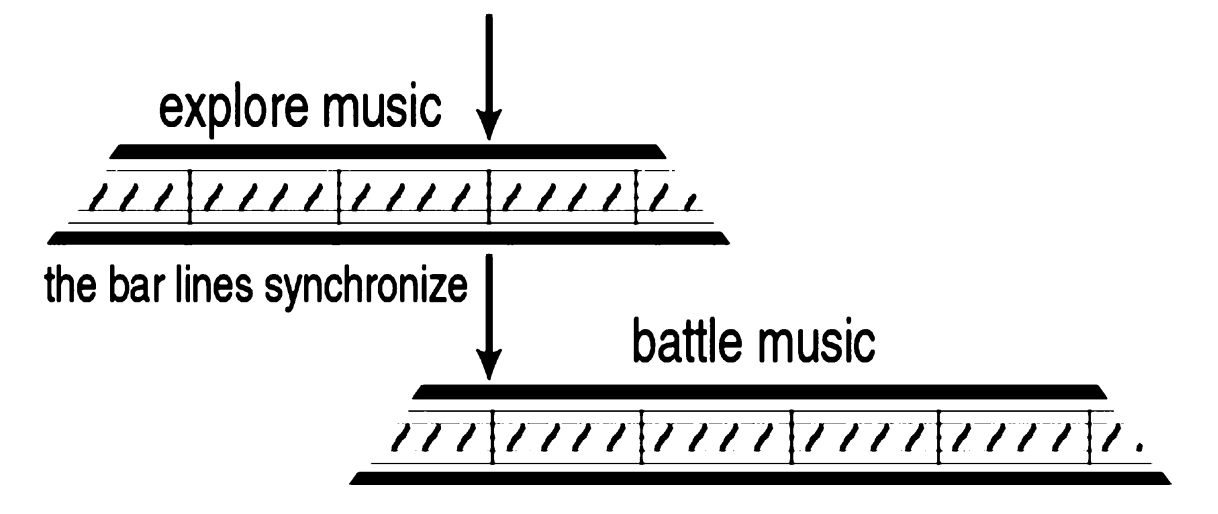
\includegraphics[width=0.4\textwidth]{img/GameMusic_SyncedScores.png}
	}
	\parbox[t]{.52\textwidth}{
		\mbox{(2) \underline{Vertical Remixing}}
			
\includegraphics[width=0.55\textwidth]{img/GameMusic_VerticalRemixing.png}
	}
	
	\medskip
	\hfill\underline{Erweiterungen}: Fade In/Out, Transitions, Score Branching, ...
	
\end{frame}

\begin{frame}[t]{VI. \dimSixTitle}{Laptopmusik, Algorave, Live Coding}

\Conclude~Nachvollziehbarkeit hier ein (künstlerisches) Problem
(analog zu serieller Musik)
\vspace{-.5cm}
\begin{center}
	\mbox{
		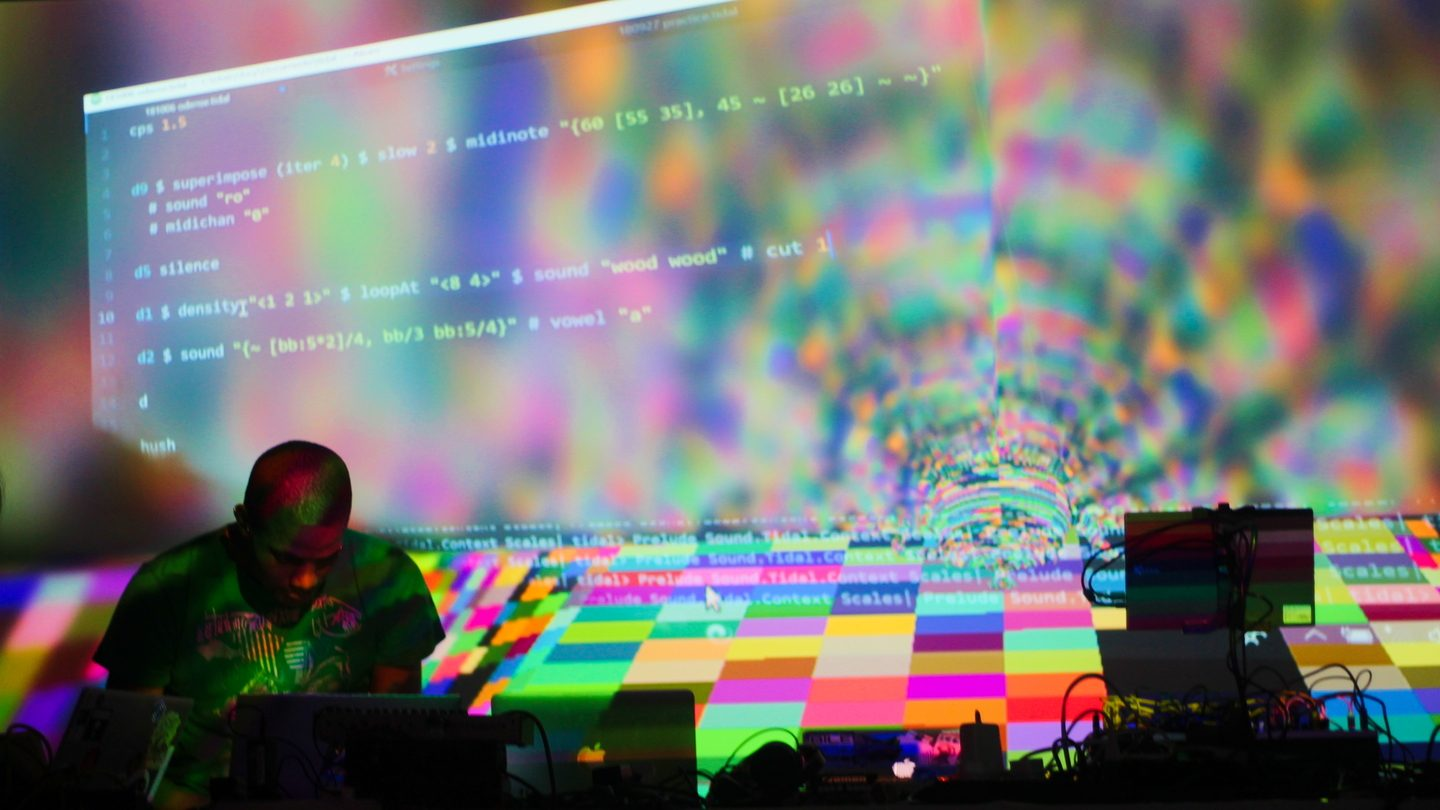
\includegraphics[width=.5\textwidth]{img/Algorave4_ByAntonioRoberts-1440x810.jpg}
		%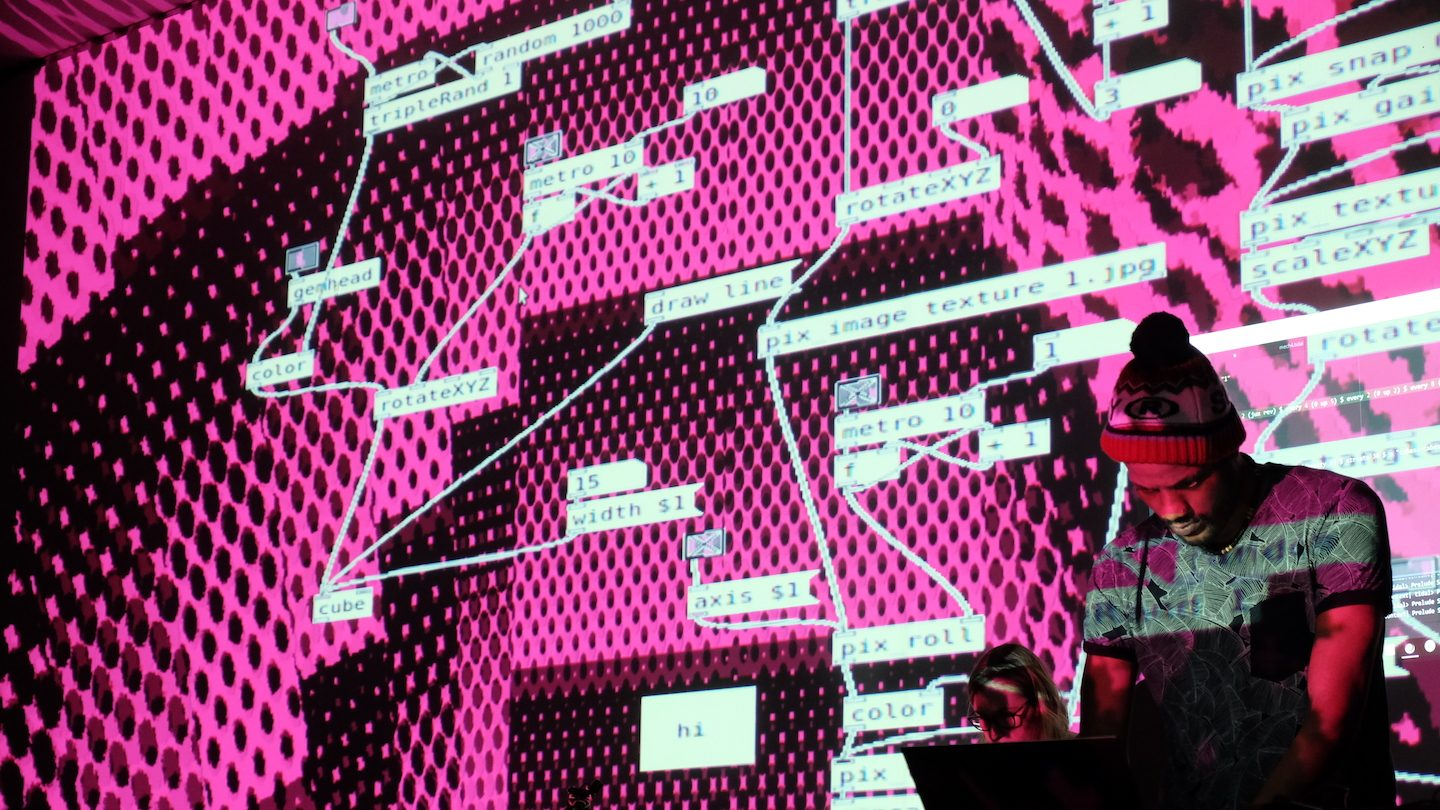
\includegraphics[width=.35\textwidth]{img/Algorave2_ByAntonioRoberts-1440x810.jpg}
		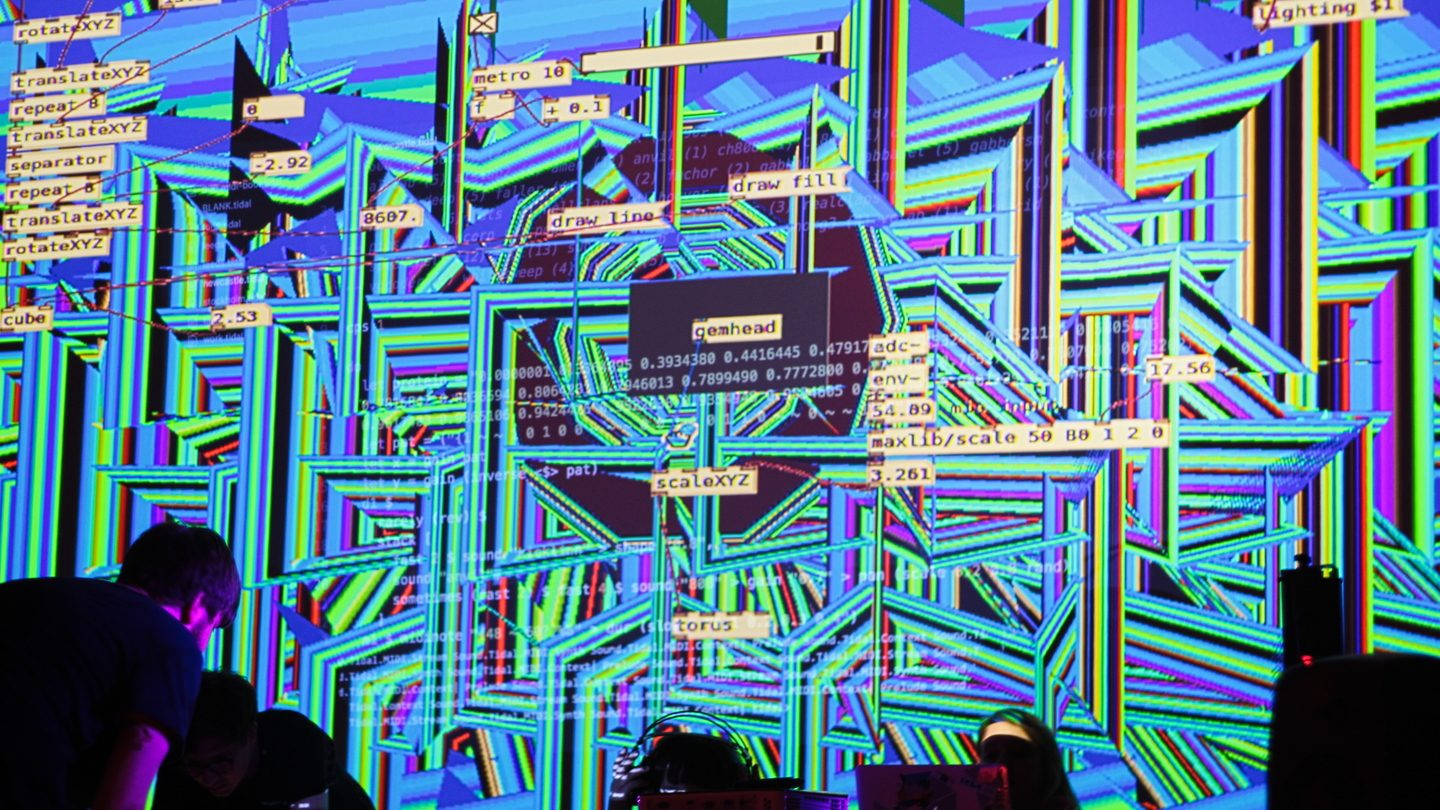
\includegraphics[width=.5\textwidth]{img/Algorave3_ByAntonioRoberts-1440x810.jpg}
	}
\end{center}

\underline{Forschung}: Conference on \textbf{AI Music Creativity}\\
\hspace{2.2cm}\url{2022.aimusiccreativity.org/}

\vspace{-1.2cm}
\tiny
\hfill \textcopyright Photos: Antonio Roberts\\
\hfill \url{noahstroehle.com/amplifying-presence}\\
\hfill \url{-algorave-at-sxsw-2019/}
\end{frame}

%%%%%%%%%%%%%%%%%%%%%%%%%%%%%%%%%%%%%%%%%%%%%%%%
%%%%%%%%%%%%%%%%%%%%%%%%%%%%%%%%%%%%%%%%%%%%%%%%
\section{Evaluation \enquote{kreativer} Systeme}

\begin{frame}{Objektive Evaluation}
%	\todobox{ein paar Maße zeigen, mit Mathe und Beispiel!!}
	
	\begin{center}
		{\Large Formalismus~~~vs.~~~Datensatzvergleich}
	\end{center}
	\bigskip

	\warnSign~Nutzen unklar\\
	\smallskip
	~~~~\conclude~Könnten Maßzahlen \enquote{Korrektheit} erlangen,\\
	\hfill wäre \emph{automatische Komposition} als \textbf{Optimierungsproblem} (z.B. EA) lösbar!\\
	\bigskip
	
	Eher: Heuristiken können notwendige Bedingungen sein, keine hinreichenden Erklärung.
\end{frame}

\begin{frame}{Subjektive Evaluation}
	\drawat{10.5cm,3cm}{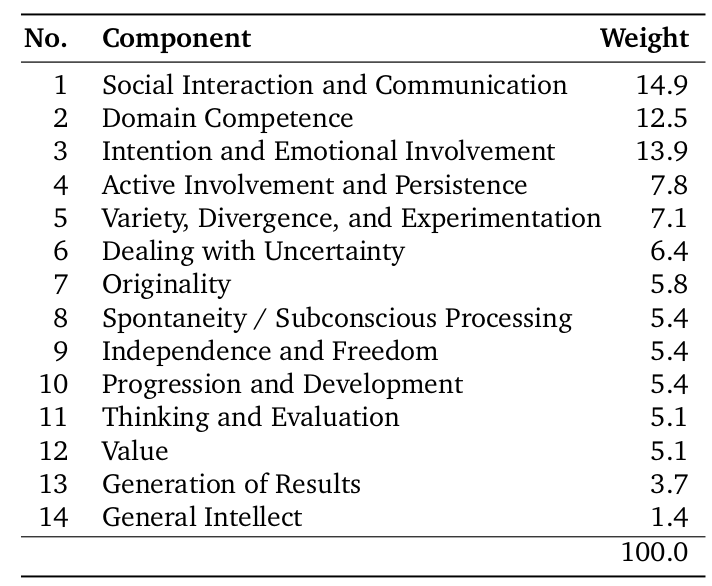
\includegraphics[height=.45\textheight]{img/SPECS_Components.png}}
	
	\underline{Möglichkeiten}
	\begin{itemize}
		\item Qualitative Befragung (z.B. Likert-Skala)
		\item Varianten von \textbf{musikalischen Turing-Tests} (\emph{Imitation Game})
		\item Standardisierte System-Evaluation, z.B. SPECS: \citep{SPECS}\\
		\medskip
		\parbox{8cm}{
			\begin{enumerate}
				\item \emph{Computational
				linguistics analysis} clustert 14 Komponenten aus akademischen Papern zum Thema \emph{creativity}
				\smallskip
				\item Verdeckte Befragung zum Begriff \enquote{musical improvisational creativity} führt zu Gewichten
			\end{enumerate}
		}
	\end{itemize}
	
	\bigskip\medskip
	\warnSign~Problematisch bei statistischen Erhebungen:\\
	\smallskip
	~~~\emph{Kategorische Ablehnung} (neg. bias) gegenüber KI-Musik\\
	\smallskip
	\conclude~kann bereits bei Ankündigung/Bewerbung einer Studie problematisch sein
\end{frame}

%%%%%%%%%%%%%%%%%%
%%%%%%%%%%%%%%%%%%
\section{Ausblick}

\begin{frame}{Aktuell im Fokus}{\enquote{Was heißt hier Intelligenz?}}
	\drawat{11.5cm,.2cm}{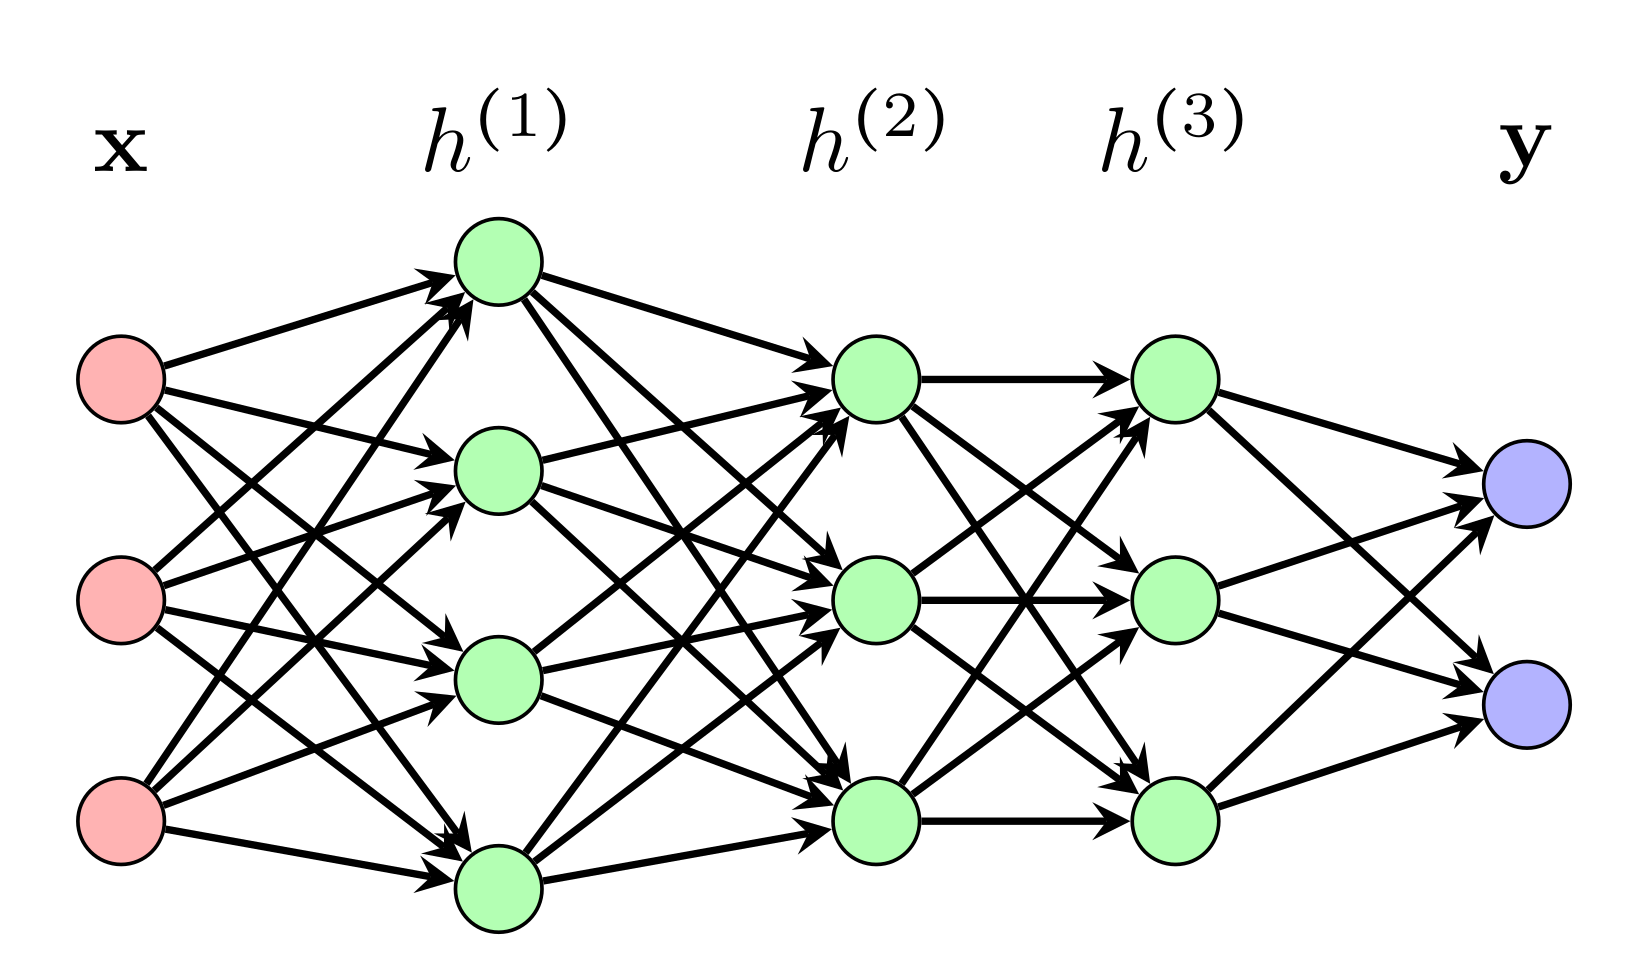
\includegraphics[width=4cm]{img/MLP-Theorie.png}}
	Die (sogenannte) \enquote{Künstliche Intelligenz} \warnSign
	\bigskip
	
	Eigentlich gemeint: \textbf{Deep Learning} = tiefe (riesige$^*$) \emph{neuronale Netze}
	\bigskip
	
	Populäre Methoden:
	\begin{itemize}
		\item Variational Auto-Encoders (VAEs)\\
			\qquad\conclude~Encoder-Decoder-Struktur
		\item Generative Adversarial Networks (GANs)\\
			\qquad\conclude~Nullsummenspiel von Generator und Diskriminator
		\item Transformer-Modelle\\
		\qquad\conclude~eigenes Thema für ein ganzes Seminar...
	\end{itemize}

	\vfill\hfill \footnotesize $^*$etwa $10^6$--$10^9$ Neuronen
\end{frame}

\begin{frame}{Deep Learning-Systeme}
		Einordnung:
		\begin{itemize}
			\item datenbasiert
			\item stochastisch\\
			~~~\conclude~{\small(deterministisch bei festem \emph{seed}; Stichwort: Pseudozufall)}
			\item (digitale) Darstellung hängt stark vom Datensatz ab\\
			~~~\conclude~{\small Score oder Sound möglich}
			\item (eher) nicht interaktiv
			\item (noch) nicht echtzeitfähig
			\item Zielsetzung: \emph{end-to-end}
		\end{itemize}
		
		\vspace{-2.2cm}
		\hfill Weiterführende Literatur: \raisebox{-\baselineskip}{\hspace{-.6cm}\citep{DL4music}~~}
		\raisebox{-1.6cm}{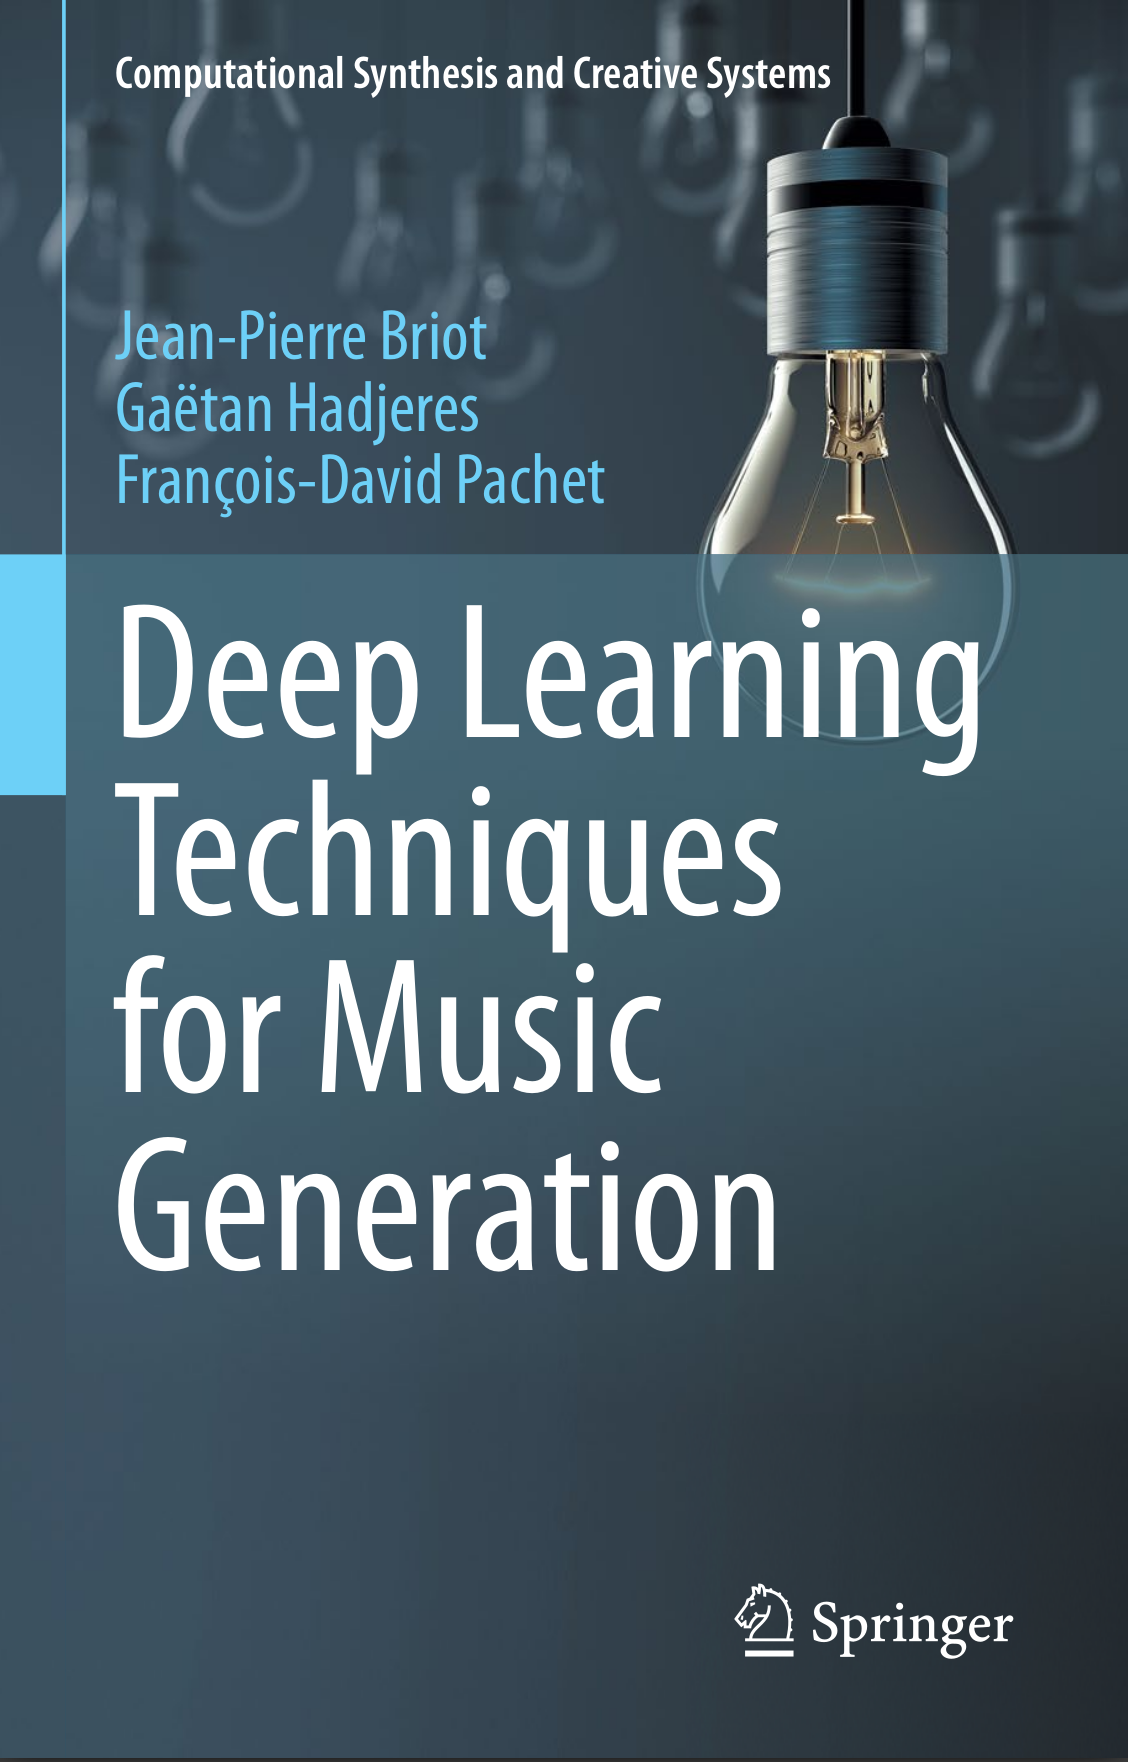
\includegraphics[height=4.5cm]{img/DL4music_cover.png}}
\end{frame}

\begin{frame}{Hierarchische Kategorisierung nach Methoden}{(Stand 2014)}
	\centering
	\includegraphics<1>[height=.75\textheight]{img/AI_Methods_For_AlgoComp_Overview.png}\includegraphics<2>[height=.8\textheight]{img/AI_Methods_For_AlgoComp_Overview_mark.png}\citep{FernandezVico2013}
\end{frame}

\begin{frame}{Die Zukunft?}{Prompt-Systeme}
	
	\underline{DALL-E 2}: \enquote{An Astronaut Riding A Horse}\\
	\smallskip
	\includegraphics[width=1.7cm]{img/Dalle2-AstronautRidingHorse/0.jpg}
	\includegraphics[width=1.7cm]{img/Dalle2-AstronautRidingHorse/1.jpg}
	\includegraphics[width=1.7cm]{img/Dalle2-AstronautRidingHorse/2.jpg}
	\includegraphics[width=1.7cm]{img/Dalle2-AstronautRidingHorse/3.jpg}
	\includegraphics[width=1.7cm]{img/Dalle2-AstronautRidingHorse/5.jpg}
	\includegraphics[width=1.7cm]{img/Dalle2-AstronautRidingHorse/7.jpg}
	\includegraphics[width=1.7cm]{img/Dalle2-AstronautRidingHorse/9.jpg}
	
	\medskip
	Video-Empfehlung:~~~ {\tiny(\url{youtube.com/watch?v=QN0DDD7B3oU})}\\
	\smallskip
	\includegraphics[width=.8\textwidth]{img/DavidBruce_Dalle2OfMusic.png}
	
	
	\hfill Spannend bleibt: \enquote{Was werden diese Systeme nicht lernen können?}\hspace{-.5cm}
	
	%TODO: Video zu ChatGPT komponiert	
\end{frame}

